% ===========================================================================
%  Bataille Navale --- rapport de projet, édition française (l'originale)
%
%  Compilation :  latexmk            (dans ce dossier)
%  Résultat    :  build/battleship-report-fr.pdf
%
%  L'édition anglaise, battleship-report-en.tex, en est la traduction : les
%  deux partagent preamble.tex, references.bib et data/.
% ===========================================================================
\documentclass[11pt, a4paper, french, oneside, parskip=half-, headings=small,
               numbers=noenddot, bibliography=totoc, listof=totoc]{scrreprt}

\newif\ifanglais \anglaisfalse
% ===========================================================================
%  Préambule : extensions, couleurs et styles du rapport
% ===========================================================================

% ------------------------------------------------------------------ langue
\usepackage[T1]{fontenc}
\usepackage[utf8]{inputenc}
\usepackage[french]{babel}
\usepackage[autostyle=true]{csquotes}

% ----------------------------------------------------------------- polices
\usepackage{libertinus}
\usepackage[scaled=0.84]{sourcecodepro}
\usepackage{microtype}

% ------------------------------------------------------------- mise en page
\usepackage[a4paper, top=2.6cm, bottom=2.8cm, left=2.7cm, right=2.7cm,
            headheight=15pt, footskip=1.2cm]{geometry}
\usepackage{scrlayer-scrpage}
\usepackage{enumitem}
\usepackage{graphicx}
\usepackage{array, booktabs, tabularx, multirow}
\usepackage{caption, subcaption}
\usepackage{float}
\usepackage[locale=FR, group-minimum-digits=4]{siunitx}

% ----------------------------------------------------------------- couleurs
\usepackage[table]{xcolor}
\definecolor{marine}{HTML}{0B3954}    % titres, traits forts
\definecolor{ocean}{HTML}{1098AD}     % accent
\definecolor{ecume}{HTML}{E3FAFC}     % fonds clairs
\definecolor{corail}{HTML}{E8590C}    % mises en garde, touches
\definecolor{sable}{HTML}{FFF4E6}     % fond des encadrés d'alerte
\definecolor{ardoise}{HTML}{495057}   % texte secondaire
\definecolor{brume}{HTML}{F1F3F5}     % fond du code
\definecolor{vert}{HTML}{2F9E44}

% ------------------------------------------------------------------ dessins
\usepackage{tikz}
\usetikzlibrary{arrows.meta, positioning, shapes.geometric, shapes.multipart,
                fit, calc, backgrounds, matrix, babel}
\usepackage{pgfplots}
\usepackage{pgfplotstable}
\usepackage[edges]{forest}
\pgfplotsset{compat=1.17}

% -------------------------------------------------------------------- code
\usepackage{listings}
\lstdefinestyle{bataille}{
  basicstyle=\ttfamily\small,
  keywordstyle=\color{marine}\bfseries,
  commentstyle=\color{ardoise}\itshape,
  stringstyle=\color{corail},
  backgroundcolor=\color{brume},
  frame=leftline, framerule=2.5pt, rulecolor=\color{ocean},
  framesep=8pt, xleftmargin=14pt, xrightmargin=4pt,
  aboveskip=10pt, belowskip=8pt,
  showstringspaces=false, columns=fullflexible, keepspaces=true,
  breaklines=true, breakatwhitespace=true, tabsize=4,
  captionpos=b, numbers=none,
  literate={é}{{\'e}}1 {è}{{\`e}}1 {ê}{{\^e}}1 {à}{{\`a}}1 {ù}{{\`u}}1 {ç}{{\c c}}1
           {ô}{{\^o}}1 {î}{{\^i}}1 {û}{{\^u}}1 {É}{{\'E}}1 {È}{{\`E}}1 {À}{{\`A}}1
           {â}{{\^a}}1 {ë}{{\"e}}1 {ï}{{\"i}}1 {œ}{{\oe}}1 {Ç}{{\c C}}1
           {→}{{$\rightarrow$}}1 {×}{{$\times$}}1 {…}{{\dots}}1
}
\lstdefinelanguage{css}{
  morekeywords={button, window, label},
  morecomment=[s]{/*}{*/}, morestring=[b]", sensitive=true
}
\lstset{style=bataille, language=C,
  morekeywords={bool, uint8_t, int8_t, uint32_t, uint64_t, bs_board, bs_ship, bs_coord,
                bs_game, bs_status, bs_knowledge, bs_rng, bs_view, bs_controller,
                bs_difficulty, bs_player, bs_cell_look, bs_turn_report, gpointer,
                bs_phase, bs_orientation, bs_view_choice, cell_context,
                GtkWidget, gboolean}}
\renewcommand{\lstlistingname}{Extrait}
\renewcommand{\lstlistlistingname}{Table des extraits de code}
\newcommand{\code}[1]{\texttt{\small #1}}

% --------------------------------------------------------------- algorithmes
\usepackage[french, ruled, vlined, linesnumbered]{algorithm2e}
\SetKwComment{Com}{$\triangleright$\ }{}
\SetCommentSty{textit}
\SetAlFnt{\small}
\DontPrintSemicolon

% ------------------------------------------------------------------ encadrés
\usepackage[most]{tcolorbox}
\newtcolorbox{retenir}[1][À retenir]{
  enhanced, colback=ecume, colframe=ocean, coltitle=white,
  fonttitle=\sffamily\bfseries\small, title={#1},
  boxrule=0pt, leftrule=3pt, arc=1.5pt, left=8pt, right=8pt, top=6pt, bottom=6pt,
  attach boxed title to top left={yshift=-2mm, xshift=3mm},
  boxed title style={colback=ocean, arc=1.5pt, boxrule=0pt, left=4pt, right=4pt}
}
\newtcolorbox{attention}[1][Défaut de la version 1]{
  enhanced, colback=sable, colframe=corail, coltitle=white,
  fonttitle=\sffamily\bfseries\small, title={#1},
  boxrule=0pt, leftrule=3pt, arc=1.5pt, left=8pt, right=8pt, top=6pt, bottom=6pt,
  attach boxed title to top left={yshift=-2mm, xshift=3mm},
  boxed title style={colback=corail, arc=1.5pt, boxrule=0pt, left=4pt, right=4pt}
}

% ---------------------------------------------------------------- titres
\addtokomafont{disposition}{\color{marine}}
\setkomafont{chapter}{\Huge\sffamily\bfseries}
\setkomafont{section}{\Large\sffamily\bfseries}
\setkomafont{subsection}{\large\sffamily\bfseries}
\setkomafont{caption}{\small}
\setkomafont{captionlabel}{\small\sffamily\bfseries\color{marine}}
\renewcommand*{\chapterformat}{%
  \textcolor{ocean}{\thechapter}\enskip\textcolor{ocean!40}{\rule[-0.15em]{1.5pt}{1em}}\enskip}
\RedeclareSectionCommand[beforeskip=0pt, afterskip=1.4\baselineskip]{chapter}

% ------------------------------------------------------- en-têtes et pieds
\clearpairofpagestyles
\ihead{\small\sffamily\color{ardoise}Bataille Navale --- rapport de projet}
\ohead{\small\sffamily\color{ardoise}\leftmark}
\cfoot{\small\sffamily\color{ardoise}\pagemark}
\KOMAoptions{headsepline=0.4pt}
\setkomafont{headsepline}{\color{ocean!50}}
\automark[chapter]{chapter}
\renewcommand*{\chaptermarkformat}{}

% ------------------------------------------------------------------- listes
\setlist{itemsep=2pt, topsep=4pt}
\setlist[itemize,1]{label={\tikz[baseline=-0.1ex]\fill[ocean] (0,0) -- (0.85ex,0.55ex) -- (0,1.1ex) -- cycle;}}
\setlist[itemize,2]{label=\textcolor{ocean}{--}}

% ------------------------------------------------------------ bibliographie
% Le moteur BibTeX suffit pour une dizaine de références et évite de dépendre de biber.
\usepackage[backend=bibtex, style=numeric, sorting=none, maxbibnames=6]{biblatex}
\addbibresource{references.bib}

% -------------------------------------------------------------------- liens
\usepackage[colorlinks=true, linkcolor=marine, urlcolor=ocean, citecolor=ocean,
            pdftitle={Bataille Navale --- rapport de projet},
            pdfauthor={Dmytro Palahin, Ivanna Makam},
            pdfsubject={Jeu de bataille navale en C11 et GTK 3},
            pdfkeywords={C11, GTK 3, MVC, bataille navale, intégration continue}]{hyperref}
\usepackage[french, nameinlink, noabbrev]{cleveref}
% Les noms propres au document sont posés après ceux que cleveref installe pour le français.
\newcommand{\nomsdesrenvois}{%
  \crefname{lstlisting}{extrait}{extraits}\Crefname{lstlisting}{Extrait}{Extraits}%
  \crefname{listing}{extrait}{extraits}\Crefname{listing}{Extrait}{Extraits}%
  \crefname{algocf}{algorithme}{algorithmes}\Crefname{algocf}{Algorithme}{Algorithmes}}
\addto\extrasfrench{\nomsdesrenvois}
\AtBeginDocument{\nomsdesrenvois}

% Les flottants restent près du texte qui les cite.
\renewcommand{\topfraction}{0.9}
\renewcommand{\bottomfraction}{0.8}
\renewcommand{\textfraction}{0.08}
\renewcommand{\floatpagefraction}{0.8}

% ------------------------------------------------------- raccourcis divers
\newcommand{\vun}{\textsf{v1}}
\newcommand{\vdeux}{\textsf{v2}}
\newcommand{\fichier}[1]{\texttt{\small #1}}
\newcommand{\depot}{\url{https://github.com/DmytroPalahin/Battleship}}
\newcommand{\touche}[1]{\tikz[baseline=(k.base)]\node[draw=ardoise, rounded corners=2pt,
  inner sep=2.5pt, font=\sffamily\scriptsize, fill=brume] (k) {#1};}

% Styles communs des schémas TikZ.
\tikzset{
  >={Stealth[length=2.2mm]},
  boite/.style={draw=marine, line width=0.7pt, rounded corners=3pt, fill=white,
                align=center, font=\sffamily\small, inner sep=6pt},
  couche/.style={boite, fill=ecume},
  coeur/.style={boite, fill=marine, text=white, draw=marine},
  externe/.style={boite, draw=ardoise, dashed, text=ardoise},
  fleche/.style={->, line width=0.7pt, draw=marine},
  note/.style={font=\sffamily\footnotesize\itshape, text=ardoise, align=center},
}

% Marque d'une case exclue par déduction, dans les figures de plateau.
\newcommand{\drapeau}[2]{%
  \node[font=\sffamily\bfseries\small, text=corail] at (#1+0.5,#2+0.5) {$\times$};}

% Quadrillage d'un plateau de côté #1 pour les figures.
\newcommand{\plateau}[1]{%
  \draw[step=1, line width=0.3pt, draw=ardoise!55] (0,0) grid (#1,#1);
  \draw[line width=0.8pt, draw=marine] (0,0) rectangle (#1,#1);}


\begin{document}

% ===========================================================================
%  Page de garde
% ===========================================================================
\begin{titlepage}
    \newgeometry{margin=0cm}
    \thispagestyle{empty}
    \begin{tikzpicture}[remember picture, overlay]
        % ---------------------------------------------------------- fond marine
        \fill[marine] (current page.north west) rectangle ([yshift=-11.2cm]current page.north east);
        \fill[ocean]  ([yshift=-11.2cm]current page.north west)
        rectangle ([yshift=-11.5cm]current page.north east);

        % ------------------------------------------------- plateau stylisé (décor)
        \begin{scope}[shift={([xshift=-8.3cm, yshift=-9.6cm]current page.north east)},
                scale=0.62, opacity=0.9]
            \draw[step=1, line width=0.3pt, draw=white!35!marine] (0,0) grid (10,10);
            \draw[line width=0.9pt, draw=ocean] (0,0) rectangle (10,10);
            % navires : 1x4, 2x3, 3x2, 4x1, sans contact
            \foreach \x/\y/\w/\h in {1/8/4/1, 7/5/1/3, 2/2/3/1, 0/5/2/1, 4/5/1/2, 8/1/2/1,
                    6/9/1/1, 9/9/1/1, 0/0/1/1, 6/3/1/1}
            \fill[ocean, rounded corners=1.5pt]
            (\x+0.12,\y+0.12) rectangle (\x+\w-0.12,\y+\h-0.12);
            % coups au but
            \foreach \x/\y in {1/8, 2/8, 7/6, 4/5}
            \fill[corail] (\x+0.5,\y+0.5) circle (0.2);
            % coups dans l'eau
            \foreach \x/\y in {3/6, 5/8, 8/3, 1/4, 6/1, 9/6, 3/0, 5/3}
            \fill[white!55!marine] (\x+0.5,\y+0.5) circle (0.1);
        \end{scope}

        % ------------------------------------------------------------- en-tête
        \node[anchor=north west, text=white, font=\sffamily\small, align=left, inner sep=0pt]
        at ([xshift=2.6cm, yshift=-2.2cm]current page.north west)
        {\textbf{Sup Galilée} --- Institut Galilée\\[2pt]
            Université Sorbonne Paris Nord};

        % --------------------------------------------------------------- titre
        \node[anchor=north west, text=white, align=left, inner sep=0pt, text width=9.2cm]
        at ([xshift=2.6cm, yshift=-4.6cm]current page.north west)
        {{\fontsize{44}{48}\selectfont\sffamily\bfseries Bataille\\[4pt] Navale}\\[18pt]
            {\Large\sffamily Du travail pratique\\[2pt] à l'architecture logicielle}};

        \node[anchor=north west, text=ocean!30, font=\sffamily, inner sep=0pt]
        at ([xshift=2.6cm, yshift=-10.2cm]current page.north west)
        {Rapport de projet \textbullet\ version 2.2};

        % ---------------------------------------------------------------- corps
        \node[anchor=north west, align=left, inner sep=0pt, text width=15.5cm]
        at ([xshift=2.6cm, yshift=-13.4cm]current page.north west)
        {{\sffamily\color{ardoise}\small Unité d'enseignement}\\[4pt]
            {\Large\sffamily\bfseries\color{marine} Initiation aux interfaces graphiques}\\[3pt]
            {\sffamily Cycle préparatoire ingénieur intégré, 2\textsuperscript{e} année
                \textbullet\ option, semestre~4}\\[3pt]
            {\sffamily Enseignante : Sophie \textsc{Toulouse}}\\[1.3cm]
            %
            {\sffamily\color{ardoise}\small Auteurs}\\[4pt]
            {\Large\sffamily\bfseries\color{marine} Dmytro \textsc{Palahin}
                \quad\textcolor{ocean}{\textbullet}\quad Ivanna \textsc{Makam}}\\[6pt]
            {\sffamily\small\color{ardoise} Projet réalisé en binôme en 2023 (version~1).\\
                Refonte de l'architecture et rédaction du présent rapport (version~2) :
                Dmytro \textsc{Palahin}, 2026.}\\[1.3cm]
            %
            {\sffamily\color{ardoise}\small Technologies}\\[4pt]
            {\sffamily C11 \textbullet\ GTK~3 \textbullet\ CMake \textbullet\ GitHub Actions}};

        % ----------------------------------------------------------------- pied
        \draw[ocean, line width=1.2pt]
        ([xshift=2.6cm, yshift=2.6cm]current page.south west) -- ++(2.2cm,0);
        \node[anchor=south west, font=\sffamily\small, text=ardoise, align=left, inner sep=0pt]
        at ([xshift=2.6cm, yshift=1.6cm]current page.south west)
        {Code source : \url{https://github.com/DmytroPalahin/battleship}\\[2pt]
            Août 2023};
    \end{tikzpicture}
    \restoregeometry
\end{titlepage}


\pagenumbering{roman}
\chapter*{Résumé}
\addcontentsline{toc}{chapter}{Résumé}

Ce rapport présente la conception et la réalisation d'un jeu de \emph{bataille navale}
contre l'ordinateur, écrit en C11 avec la bibliothèque graphique GTK~3.

Le projet est né en 2023 d'un travail en binôme pour le cours \emph{Initiation aux interfaces
    graphiques}. La première version tenait dans un unique fichier de \num{2666} lignes : le jeu
fonctionnait, mais les règles, l'affichage et les réactions aux clics y étaient mêlés, et
chacun des trois niveaux de difficulté était une copie du même code.

La seconde version, objet de ce document, conserve le jeu et en refait les fondations. Elle
applique jusqu'au bout l'organisation \emph{modèle / vue / contrôleur} enseignée dans le
cours :

\begin{itemize}
    \item un \textbf{moteur de jeu} autonome, bibliothèque C11 sans aucune dépendance, sans
          allocation dynamique et sans état global ;
    \item \textbf{deux interfaces} pour ce même moteur, l'une graphique (GTK~3), l'autre en
          mode terminal --- preuve que le modèle ignore réellement sa vue ;
    \item \textbf{trois adversaires} dont la force est \emph{mesurée} sur des milliers de
          parties reproductibles : il faut en moyenne \num{96.2}, \num{65.8} et \num{55.3}
          tirs aux niveaux facile, moyen et difficile pour couler une flotte ;
    \item une \textbf{chaîne de qualité} complète : 54 cas de test unitaires, des tests de
          propriétés rejouant \num{2250} parties, un test de bout en bout de l'interface,
          l'analyse statique et dynamique du code, l'intégration et la livraison continues.
\end{itemize}

Le rapport décrit l'architecture retenue, les structures de données et les algorithmes ---
placement aléatoire d'une flotte, déductions tirées de la règle de non-contact, carte de
probabilité du niveau difficile ---, puis la démarche de vérification. Il se termine par un
bilan chiffré comparant les deux versions.

\vspace{1.2em}
\noindent\textbf{Mots-clés :} langage C, GTK, modèle-vue-contrôleur, programmation
modulaire, intelligence artificielle de jeu, tests, intégration continue.

\chapter*{Abstract}
\addcontentsline{toc}{chapter}{Abstract}

\begin{otherlanguage}{english}
    This report describes the design and implementation of a \emph{Battleship} game against the
    computer, written in C11 with the GTK~3 toolkit.

    The project started in 2023 as a pair assignment: a single \num{2666}-line file in which
    rules, display and event handling were intertwined. Version~2 keeps the game and rebuilds its
    foundations on a strict model / view / controller architecture: a dependency-free game engine,
    a graphical and a terminal front-end sharing it, three computer opponents whose strength is
    measured over thousands of reproducible games (\num{96.2}, \num{65.8} and \num{55.3} shots on
    average to sink a fleet), and a complete quality pipeline --- unit and property tests, an
    end-to-end interface test, static and dynamic analysis, continuous integration and delivery.
\end{otherlanguage}


{\hypersetup{linkcolor=marine}
    \setcounter{tocdepth}{1}
    \tableofcontents}

\cleardoublepage
\pagenumbering{arabic}

\chapter{Introduction}
\label{chap-introduction}

\section{Contexte}

Le cours \emph{Initiation aux interfaces graphiques} de Sup Galilée~\cite{toulouse2023}
s'achève par un projet : doter d'une interface graphique, avec la bibliothèque GTK, un jeu
de bataille navale. Le cours ne se réduit pas à l'apprentissage des fenêtres et des boutons.
Il défend une idée d'organisation, la \emph{programmation modulaire}, que ses supports
reprennent d'une séance à l'autre et que l'on peut résumer ainsi :

\begin{itemize}
    \item à chaque concept, un fichier d'en-tête qui en donne la définition et le mode
          d'emploi, et un fichier source qui en réalise les fonctions de manipulation ;
    \item l'utilisation d'un concept est indépendante de sa réalisation ;
    \item un même programme peut recevoir plusieurs interfaces --- console, fenêtre --- et
          c'est alors la seule partie qui doit changer ;
    \item toute fonction écrite est aussitôt testée.
\end{itemize}

De là découle le découpage d'une application en trois bibliothèques : le \emph{modèle}, qui
représente le jeu et ses règles ; la \emph{vue}, qui regroupe les composants graphiques ;
le \emph{contrôleur}, \enquote{chef d'orchestre qui fait le lien entre les deux}.

\section{La première version}

En 2023, nous avons réalisé ce projet en binôme. Plutôt que d'habiller la bibliothèque
fournie, nous avions choisi d'écrire l'intégralité du jeu, pour mieux nous approprier GTK.
Le résultat était un jeu complet et agréable : trois niveaux de difficulté, un placement
aléatoire des flottes, des écrans de règles et de présentation, une identité visuelle
soignée.

Mais ce jeu tenait dans \emph{un seul fichier} de \num{2666} lignes, et son organisation
contredisait ce que le cours enseignait :

\begin{itemize}
    \item l'état de la partie était réparti entre sept variables globales et les composants
          graphiques eux-mêmes : la structure décrivant une case contenait à la fois
          \enquote{y a-t-il un bateau ?} et l'adresse du bouton qui l'affiche ;
    \item les trois niveaux étaient trois copies d'une même fonction de plusieurs centaines de
          lignes ; une correction faite dans l'une manquait dans les autres ;
    \item aucune règle ne pouvait s'exécuter sans ouvrir une fenêtre, donc aucun test
          automatique n'était possible ;
    \item le programme ne fonctionnait que lancé depuis son propre dossier, et sa variante
          sonore que sur la machine où elle avait été écrite.
\end{itemize}

Le programme \emph{marchait}. Il n'était ni vérifiable, ni modifiable sans risque, ni
réutilisable.

\section{Objectifs de la refonte}

La version~2 a un objectif simple à énoncer : \textbf{garder le jeu, refaire tout le reste}.
Le joueur doit retrouver les mêmes règles, les mêmes écrans, les mêmes textes. Sous la
surface, le programme doit devenir ce qu'un logiciel entretenu dans la durée doit être :

\begin{enumerate}
    \item \textbf{modulaire} --- un modèle réellement indépendant de l'interface, au point de
          pouvoir être piloté par une seconde interface ;
    \item \textbf{vérifié} --- des tests automatiques pour les règles, les stratégies de
          l'ordinateur et l'interface elle-même ;
    \item \textbf{reproductible} --- une partie entièrement déterminée par une graine, une
          compilation identique sur un poste de travail et sur un serveur ;
    \item \textbf{livrable} --- un exécutable unique, des paquets, une intégration et une
          livraison continues.
\end{enumerate}

\section{Organisation du rapport}

Le \cref{chap-exigences} fixe les règles du jeu et les exigences. Le
\cref{chap-architecture} présente l'architecture et la justifie. Les
\cref{chap-modele,chap-adversaire} détaillent le moteur de jeu puis l'adversaire
artificiel, avec les mesures de sa force. Le \cref{chap-interface} décrit l'interface
graphique. Le \cref{chap-qualite} expose la démarche de vérification et la chaîne
d'intégration continue. Le \cref{chap-bilan} dresse le bilan chiffré de la refonte, ses
limites et ses prolongements possibles.

\chapter{Le jeu et ses exigences}
\label{chap-exigences}

\section{Règles}

Le joueur commande la flotte de la \emph{Sup Galilée Marine Nationale} contre une flotte de
pirates dirigée par l'ordinateur. Chaque camp dispose d'une grille de $10 \times 10$ cases et
d'une flotte de dix bateaux, soit vingt cases occupées (\cref{tab-flotte}).

\begin{table}[ht]
    \centering
    \begin{tabular}{@{}lccc@{}}
        \toprule
        Type de bateau  & Longueur (cases) & Nombre      & Cases occupées \\
        \midrule
        Quatre ponts    & 4                & 1           & 4              \\
        Trois ponts     & 3                & 2           & 6              \\
        Deux ponts      & 2                & 3           & 6              \\
        Un pont         & 1                & 4           & 4              \\
        \midrule
        \textbf{Flotte} &                  & \textbf{10} & \textbf{20}    \\
        \bottomrule
    \end{tabular}
    \caption{Composition d'une flotte.}
    \label{tab-flotte}
\end{table}

\begin{description}[style=nextline, leftmargin=1.2em]
    \item[Placement] Les bateaux sont droits, horizontaux ou verticaux. Deux bateaux ne se
          touchent jamais, \emph{ni par un côté, ni par un coin} : chaque bateau est entouré d'une
          ceinture d'eau (\cref{fig-non-contact}). Les flottes sont placées au hasard ; le joueur
          peut faire retirer la sienne tant qu'aucun coup n'a été tiré.
    \item[Tour de jeu] Le joueur commence. Tirer consiste à désigner une case de la grille
          adverse. Si un bateau s'y trouve, il est \emph{touché} et le tireur rejoue ; sinon le
          tir est \emph{manqué} et la main passe.
    \item[Bateau coulé] Un bateau dont toutes les cases sont touchées est \emph{coulé}.
    \item[Fin de partie] Le premier camp dont la flotte entière est coulée a perdu.
\end{description}

\begin{figure}[ht]
    \centering
    \begin{tikzpicture}[scale=0.62]
        % ------------------------------------------------ (a) placement licite
        \begin{scope}
            \fill[ecume] (1,2) rectangle (6,5);
            \plateau{7}
            \fill[marine, rounded corners=1.5pt] (2.12,3.12) rectangle (4.88,3.88);
            \fill[ocean, rounded corners=1.5pt] (6.12,0.12) rectangle (6.88,1.88);
            \fill[ocean, rounded corners=1.5pt] (0.12,6.12) rectangle (1.88,6.88);
            \node[note] at (3.5,-0.8) {(a) ceinture d'eau d'un bateau\\et voisins licites};
        \end{scope}
        % ---------------------------------------------- (b) placements interdits
        \begin{scope}[xshift=9.5cm]
            \plateau{7}
            \fill[marine, rounded corners=1.5pt] (2.12,3.12) rectangle (4.88,3.88);
            \fill[corail, rounded corners=1.5pt] (5.12,4.12) rectangle (5.88,5.88);
            \fill[corail, rounded corners=1.5pt] (1.12,2.12) rectangle (3.88,2.88);
            \draw[corail, line width=1.2pt] (4.75,3.75) -- (5.25,4.25) (4.75,4.25) -- (5.25,3.75);
            \draw[corail, line width=1.2pt] (2.75,2.75) -- (3.25,3.25) (2.75,3.25) -- (3.25,2.75);
            \node[note] at (3.5,-0.8) {(b) contact par un coin\\et contact par un côté};
        \end{scope}
    \end{tikzpicture}
    \caption{La règle de non-contact. En (a), la zone claire est interdite aux autres
        bateaux ; en (b), deux placements refusés.}
    \label{fig-non-contact}
\end{figure}

La règle de non-contact a une conséquence qui structure tout le projet : elle permet de
\emph{déduire}. Un coup au but prouve que ses quatre voisines diagonales sont de l'eau ; un
bateau coulé prouve que toute sa ceinture l'est aussi. Le jeu signale ces cases par un
drapeau, et la force de l'adversaire artificiel dépend d'abord de l'usage qu'il fait de ces
déductions (\cref{chap-adversaire}).

\section{Exigences fonctionnelles}

\begin{table}[ht]
    \centering
    \begin{tabularx}{\textwidth}{@{}lX@{}}
        \toprule
        \textbf{F1} & Jouer une partie complète contre l'ordinateur, selon les règles ci-dessus.   \\
        \textbf{F2} & Choisir parmi trois niveaux de difficulté : facile, moyen, difficile.        \\
        \textbf{F3} & Placer les flottes au hasard ; retirer celle du joueur avant le premier tir. \\
        \textbf{F4} & Afficher l'état des deux grilles : bateaux du joueur, tirs manqués, coups
        au but, bateaux coulés, cases exclues par déduction.                                       \\
        \textbf{F5} & Afficher le score de chaque camp et le tour en cours.                        \\
        \textbf{F6} & Consulter les règles et la présentation du jeu à tout moment.                \\
        \textbf{F7} & En fin de partie, proposer de rejouer, de changer de niveau ou de quitter.   \\
        \textbf{F8} & Jouer au clavier comme à la souris ; effets sonores facultatifs.             \\
        \bottomrule
    \end{tabularx}
    \caption{Exigences fonctionnelles.}
    \label{tab-fonctionnelles}
\end{table}

\section{Exigences de conception}

Ce sont elles qui distinguent la version~2 de la première. Chacune est vérifiable, et le
\cref{chap-qualite} montre par quel moyen elle l'est effectivement.

\begin{table}[ht]
    \centering
    \begin{tabularx}{\textwidth}{@{}lXl@{}}
        \toprule
                    & \textbf{Exigence}                                                        & \textbf{Vérifiée par} \\
        \midrule
        \textbf{C1} & Le modèle ne dépend ni de GTK ni d'aucune autre bibliothèque.            &
        compilation sans GTK                                                                                           \\
        \textbf{C2} & Une même graine rejoue exactement la même partie, sur toute plate-forme. &
        fichier de référence                                                                                           \\
        \textbf{C3} & L'adversaire ne peut pas tricher : il ignore la position des bateaux.    &
        construction (types)                                                                                           \\
        \textbf{C4} & Une opération refusée laisse l'état du jeu intact.                       & tests unitaires       \\
        \textbf{C5} & Aucun avertissement du compilateur ; aucune erreur mémoire.              &
        \code{-Werror}, ASan, UBSan                                                                                    \\
        \textbf{C6} & Le programme se lance depuis n'importe quel dossier.                     &
        ressources incorporées                                                                                         \\
        \textbf{C7} & L'interface ne se fige jamais pendant le tour de l'ordinateur.           &
        un tir par tic d'horloge                                                                                       \\
        \bottomrule
    \end{tabularx}
    \caption{Exigences de conception et moyens de vérification.}
    \label{tab-conception}
\end{table}

\chapter{Architecture}
\label{chap-architecture}

\section{Une seule règle : les dépendances pointent vers l'intérieur}

L'architecture tient en une phrase : \textbf{le moteur de jeu ne sait pas comment il est
    affiché ; les interfaces connaissent le moteur ; rien ne connaît les interfaces}
(\cref{fig-couches}).

\begin{figure}[ht]
    \centering
    \begin{tikzpicture}[node distance=7mm and 9mm]
        \node[coeur, minimum width=11.2cm, minimum height=1.5cm] (core)
        {\textbf{battleship\_core} --- moteur de jeu (le \emph{modèle})\\[2pt]
            \footnotesize C11, bibliothèque standard seule, aucune allocation dynamique};

        \node[couche, above=14mm of core.north west, anchor=south west, minimum width=3.4cm,
            minimum height=1.6cm] (gui)
        {\textbf{battleship}\\[1pt]\footnotesize application GTK~3\\\footnotesize vue + contrôleur};
        \node[couche, above=14mm of core.north, anchor=south, minimum width=3.4cm,
            minimum height=1.6cm] (cli)
        {\textbf{battleship-cli}\\[1pt]\footnotesize jeu en terminal\\\footnotesize simulateur};
        \node[couche, above=14mm of core.north east, anchor=south east, minimum width=3.4cm,
            minimum height=1.6cm] (tests)
        {\textbf{tests}\\[1pt]\footnotesize unitaires\\\footnotesize et de propriétés};

        \node[externe, above=9mm of gui, minimum width=3.4cm] (gtk) {GTK~3, GLib\\[-1pt]
            \footnotesize GStreamer (facultatif)};

        \draw[fleche] (gui.south) -- (gui.south |- core.north);
        \draw[fleche] (cli.south) -- (core.north);
        \draw[fleche] (tests.south) -- (tests.south |- core.north);
        \draw[fleche, draw=ardoise, dashed] (gui.north) -- (gtk.south);

        \node[note, right=5mm of gtk, text width=6.4cm, align=left]
        {Une flèche se lit \enquote{dépend de}.\\Aucune ne part du moteur.};
    \end{tikzpicture}
    \caption{Les couches du programme. Trois exécutables sont construits sur le même moteur.}
    \label{fig-couches}
\end{figure}

Cette règle n'est pas une convention que l'on se promet de respecter : elle est
\emph{imposée par la construction}. Le moteur est une bibliothèque statique dont le seul
chemin d'inclusion est le dossier \fichier{include/}. La chaîne d'intégration continue le
compile et le teste dans un conteneur où GTK n'est pas installé (\cref{sec-ci}) : si quelqu'un
ajoutait au moteur un appel à GTK, cette étape cesserait de compiler.

Trois programmes s'appuient sur le moteur. En avoir plus d'un n'est pas un luxe. Tant qu'il
n'existe qu'une interface, rien ne prouve que le modèle en soit indépendant ; la seconde
interface en est la démonstration.

\section{Du cours au projet : modèle, vue, contrôleur}

Le découpage \emph{modèle / vue / contrôleur} est né à la fin des années 1970 dans
l'environnement Smalltalk~\cite{reenskaug1979, krasner1988}. Il sépare ce qu'un programme
\emph{sait}, ce qu'il \emph{montre} et la façon dont il \emph{réagit}.

Le cours décrit le fonctionnement d'une application graphique en trois temps~\cite{toulouse2023} :
l'utilisateur agit sur la vue, l'action correspondante se déroule dans le modèle, puis la vue
est mise à jour. Il en tire trois bibliothèques. Le \cref{tab-mvc} montre comment le
projet les réalise.

\begin{table}[ht]
    \centering
    \begin{tabularx}{\textwidth}{@{}l>{\raggedright\arraybackslash}X>{\raggedright\arraybackslash}X@{}}
        \toprule
                            & \textbf{Rôle (cours)}                                                  & \textbf{Réalisation (projet)} \\
        \midrule
        \textbf{Modèle}     & Types utilisateur et fonctions de manipulation : le jeu et ses règles. &
        \fichier{include/battleship/}, \fichier{src/core/} --- plateau, tirs, déductions,
        tour de jeu, adversaire.                                                                                                     \\
        \addlinespace
        \textbf{Vue}        & Composants graphiques à organiser dans des fenêtres.                   &
        \fichier{src/ui/view.c} --- tous les \emph{widgets}, aucune règle ;
        \fichier{assets/style.css} pour l'apparence.                                                                                 \\
        \addlinespace
        \textbf{Contrôleur} & Chef d'orchestre : associe les actions aux événements,
        synchronise la vue. &
        \fichier{src/ui/controller.c} --- demande au modèle de jouer, puis resynchronise
        la vue.                                                                                                                      \\
        \bottomrule
    \end{tabularx}
    \caption{Correspondance entre l'organisation du cours et celle du projet.}
    \label{tab-mvc}
\end{table}

\subsection{Qui possède quoi ?}

Le cours discute quatre façons de regrouper le modèle et la vue dans la structure du
contrôleur, et retient celle où le modèle est \emph{référencé} et la vue \emph{possédée} :
le modèle a une existence propre, antérieure et postérieure à toute interface graphique,
alors que la vue n'a de raison d'être qu'avec son contrôleur. Le projet fait exactement ce
choix (\cref{lst-controleur})\footnote{Dans les extraits de la version~2, les commentaires,
    rédigés en anglais dans le code, sont traduits ; certains sont abrégés.}.

\begin{lstlisting}[caption={La structure du contrôleur (\fichier{src/ui/controller.c}).},
                   label={lst-controleur}]
struct bs_controller {
    GtkApplication *application;
    bs_game *model; /* emprunté : appartient à l'application */
    bs_view *view;  /* possédé  : construit et détruit par le contrôleur */
    /* ... */
};
\end{lstlisting}

Le modèle, lui, est déclaré par l'application (\fichier{src/ui/app.c}), en dehors du
contrôleur. Il pourrait être sauvegardé, rejoué ou confié à une autre interface sans que
l'interface graphique en sache rien.

\subsection{La variante \enquote{à pointeurs de fonctions}}
\label{sec-pointeurs}

Dans le corrigé du cours, le contrôleur va chercher les boutons dans la vue
(\code{vue\_tresor\_get\_boite()}) et leur attache lui-même les fonctions de rappel. Une note
ajoute qu'une autre voie, plus élégante, existe au prix de pointeurs de fonctions. C'est
cette variante que le projet met en œuvre.

La vue connecte elle-même ses signaux et traduit chaque geste de l'utilisateur en une
\emph{intention}, exprimée dans le vocabulaire du jeu, qu'elle transmet par une table de
fonctions de rappel (\cref{lst-actions}).

\begin{lstlisting}[caption={Les intentions rapportées par la vue (\fichier{src/ui/view.h}).},
                   label={lst-actions}]
typedef struct bs_view_actions {
    void (*level_chosen)(bs_difficulty level, gpointer user_data);
    void (*cell_activated)(bs_coord cell, gpointer user_data);
    void (*reshuffle_requested)(gpointer user_data);
    void (*restart_requested)(gpointer user_data);
    void (*quit_requested)(gpointer user_data);
    void (*game_over_answered)(bs_view_choice choice, gpointer user_data);
    void (*closed)(gpointer user_data);
} bs_view_actions;
\end{lstlisting}

La conséquence est forte : \textbf{aucun \code{GtkWidget} ne franchit l'interface de la
    vue}. Le contrôleur ne manipule pas de boutons ; il dit \emph{quoi} montrer --- \enquote{cette
    case est un coup au but} --- jamais \emph{comment}. Il pourrait piloter une tout autre
bibliothèque graphique sans changer d'une ligne.

\section{Les modules}

\begin{figure}[ht]
    \centering
    \begin{tikzpicture}[node distance=6mm]
        \node[boite] (types) {\textbf{types}\\[-1pt]\footnotesize coordonnées,\\[-2pt]\footnotesize statuts};
        \node[boite, right=of types] (rng) {\textbf{rng}\\[-1pt]\footnotesize hasard\\[-2pt]\footnotesize reproductible};
        \node[boite, right=of rng] (board) {\textbf{board}\\[-1pt]\footnotesize flotte, tirs,\\[-2pt]\footnotesize déductions};
        \node[boite, right=of board] (ai) {\textbf{ai}\\[-1pt]\footnotesize choix\\[-2pt]\footnotesize d'une cible};
        \node[boite, right=of ai] (game) {\textbf{game}\\[-1pt]\footnotesize tour de jeu,\\[-2pt]\footnotesize score, fin};
        \draw[fleche] (rng) -- (types);
        \draw[fleche] (board) -- (rng);
        \draw[fleche] (ai) -- (board);
        \draw[fleche] (game) -- (ai);
    \end{tikzpicture}
    \caption{Les modules du moteur forment une chaîne : chacun ne s'appuie que sur les
        précédents.}
    \label{fig-modules}
\end{figure}

À l'intérieur du moteur, les cinq modules forment une chaîne stricte (\cref{fig-modules}).
Chacun suit le patron du cours : un fichier d'en-tête qui fixe les responsabilités ---
structure de données, mode d'emploi, pré-conditions --- et un fichier source qui les réalise. Le \cref{tab-arborescence} donne l'organisation complète du dépôt.

\begin{table}[ht]
    \centering
    \small
    \begin{tabularx}{\textwidth}{@{}l>{\raggedright\arraybackslash}Xr@{}}
        \toprule
        \textbf{Dossier}                                   & \textbf{Contenu}                                           & \textbf{Lignes} \\
        \midrule
        \fichier{include/battleship/}, \fichier{src/core/} & Moteur de jeu : interface publique et réalisation          & \num{1343}      \\
        \fichier{src/cli/}                                 & Interface terminal et simulateur                           & \num{645}       \\
        \fichier{src/ui/}                                  & Application GTK : vue, contrôleur, coquille, son           & \num{1670}      \\
        \fichier{assets/}                                  & Images, sons, feuille de style (incorporés à l'exécutable) & \num{199}       \\
        \fichier{tests/}                                   & Tests unitaires, de propriétés et de l'interface terminal  & \num{1582}      \\
        \fichier{docs/}                                    & Guide d'architecture, décisions, présent rapport           &                 \\
        \fichier{cmake/}, \fichier{packaging/}             & Modules de construction, intégration au bureau             &                 \\
        \fichier{.github/}                                 & Intégration et livraison continues                         &                 \\
        \bottomrule
    \end{tabularx}
    \caption{Organisation du dépôt. Les lignes comptent le code et ses commentaires ;
        pour \fichier{assets/}, la feuille de style seule.}
    \label{tab-arborescence}
\end{table}

\begin{retenir}
    Le code des tests (\num{1582} lignes) est plus volumineux que celui du moteur qu'il vérifie
    (\num{1343} lignes, en-têtes compris). Ce rapport est habituel pour un composant dont on
    veut pouvoir garantir le comportement.
\end{retenir}

\chapter{Le modèle : un moteur de jeu autonome}
\label{chap-modele}

Le modèle est une bibliothèque de \num{1343} lignes, écrite en C11~\cite{iso9899}, qui connaît
les règles de la bataille navale et rien d'autre. Ce chapitre en présente les structures de données, puis les
traitements, dans l'ordre de la chaîne de modules de la \cref{fig-modules}.

\section{Représenter un plateau}

Dans la version~1, une case était décrite par une structure mêlant l'état du jeu et
l'affichage (\cref{lst-v1-cell}). Tester si un bateau était coulé supposait d'avoir construit
des boutons.

\begin{lstlisting}[caption={Version~1 : la case connaît son bouton.}, label={lst-v1-cell}]
typedef struct {
    GtkWidget *button;  // Button to display the cell
    gboolean is_ship;   // Flag indicating whether there is a ship in this box
    gboolean is_hit;
    gboolean is_shot;
} Cell;
\end{lstlisting}

La version~2 sépare deux natures d'information que la première confondait : le
\textbf{secret} --- où sont les bateaux --- et ce qui est \textbf{public} --- ce que les
tirs ont révélé (\cref{lst-board}).

\begin{lstlisting}[caption={Le plateau d'un camp (\fichier{include/battleship/board.h}).},
                   label={lst-board}]
typedef struct bs_ship {
    bs_coord origin;            /* pont le plus en haut à gauche */
    bs_orientation orientation; /* direction des ponts suivants   */
    uint8_t length;             /* nombre de ponts, de 1 à 4      */
    uint8_t hits;               /* ponts déjà touchés             */
} bs_ship;

typedef struct bs_board {
    bs_ship ships[BS_FLEET_SIZE];
    uint8_t ship_count;            /* bateaux placés                    */
    uint8_t ships_afloat;          /* bateaux non coulés                */
    uint8_t decks_afloat;          /* ponts non touchés                 */
    int8_t  ship_at[BS_CELL_COUNT]; /* secret : indice du bateau, ou -1 */
    uint8_t state[BS_CELL_COUNT];   /* public : ce que la case a révélé */
} bs_board;
\end{lstlisting}

L'état public d'une case prend l'une des cinq valeurs du \cref{tab-etats}. La cinquième,
\code{EXCLUDED}, n'existait pas dans la version~1 comme donnée : elle n'apparaissait que
sous la forme d'un drapeau posé sur un bouton.

\begin{table}[ht]
    \centering
    \begin{tabularx}{\textwidth}{@{}lX@{}}
        \toprule
        \textbf{État}             & \textbf{Signification pour l'attaquant}             \\
        \midrule
        \code{BS\_CELL\_UNKNOWN}  & Jamais visée, rien n'est connu.                     \\
        \code{BS\_CELL\_MISS}     & Visée : de l'eau.                                   \\
        \code{BS\_CELL\_HIT}      & Visée : pont d'un bateau encore à flot.             \\
        \code{BS\_CELL\_SUNK}     & Visée : pont d'un bateau coulé.                     \\
        \code{BS\_CELL\_EXCLUDED} & Non visée, mais \emph{prouvée} vide par la règle de
        non-contact.                                                                    \\
        \bottomrule
    \end{tabularx}
    \caption{États publics d'une case.}
    \label{tab-etats}
\end{table}

\begin{retenir}[Invariants du plateau]
    Toutes les fonctions du module préservent trois propriétés, que les tests de propriétés
    revérifient après chaque tir de \num{2250} parties (\cref{sec-proprietes}) :
    \begin{itemize}
        \item les bateaux ne se chevauchent pas, ne se touchent pas et ne sortent pas du plateau ;
        \item \code{decks\_afloat} est égal au nombre de ponts non encore touchés ;
        \item une case est \code{SUNK} si et seulement si elle appartient à un bateau dont tous
              les ponts sont touchés.
    \end{itemize}
\end{retenir}

\subsection{Aucune allocation dynamique}

Les dimensions du jeu sont fixes : tout tient dans des tableaux de taille connue à la
compilation. Une partie entière, \code{bs\_game}, occupe 800~octets. Le moteur n'appelle
jamais \code{malloc}. Il n'y a donc ni échec d'allocation à traiter, ni fuite possible, et
copier une partie se réduit à une affectation. C'est ce qui rend bon marché l'exécution de
millions de parties simulées.

\section{Placer une flotte au hasard}

\subsection{L'algorithme de la version~1 : tirer jusqu'à ce que ça rentre}

La première version tirait une position et une orientation au hasard, vérifiait si le
bateau tenait, et recommençait sinon, jusqu'à un million de tentatives. La méthode
fonctionne, mais sa durée n'est pas bornée de façon utile et son test de validité comportait
une erreur de borne, masquée par le choix des intervalles de tirage.

\subsection{L'algorithme de la version~2 : énumérer, puis choisir}

Pour chaque bateau, du plus long au plus court, on dresse la liste de \emph{toutes} les
positions licites, puis on en choisit une uniformément (\cref{alg-placement}). Une grille
de 100 cases et deux orientations donnent au plus 200 candidats : l'énumération est
immédiate, et l'algorithme ne dépend plus de la chance pour terminer.

\begin{algorithm}[ht]
    \caption{Placement aléatoire d'une flotte}
    \label{alg-placement}
    \KwIn{un générateur aléatoire $g$}
    \KwOut{un plateau portant les dix bateaux, sans contact}
    \Repeat{la flotte est complète}{
        vider le plateau\;
        \ForEach{longueur $\ell$ de la flotte, dans l'ordre $4, 3, 3, 2, 2, 2, 1, 1, 1, 1$}{
            $P \gets$ ensemble des couples (origine, orientation) où un bateau de longueur $\ell$
            tient sans toucher un bateau déjà placé\;
            \lIf{$P = \emptyset$}{abandonner cette tentative \Com*[f]{impasse}}
            choisir $p \in P$ uniformément avec $g$ et placer le bateau en $p$\;
        }
    }
\end{algorithm}

Le test \enquote{tient sans toucher} est une simple inspection : on parcourt le rectangle
occupé par le bateau, agrandi d'une case dans toutes les directions, et l'on refuse la
position dès qu'une case de ce rectangle porte déjà un bateau. Un bateau d'un seul pont est
identique dans les deux orientations ; il n'est compté qu'une fois, pour ne pas fausser le
tirage.

Une impasse --- plus aucune place pour un bateau restant --- est théoriquement possible.
Elle ne s'est produite dans aucune des flottes tirées par les tests, soit plusieurs
dizaines de milliers ; la boucle externe, bornée à mille tentatives, ne sert qu'à transformer un
\enquote{ne peut pas arriver} en erreur signalée plutôt qu'en boucle sans fin.

\section{Tirer, et en tirer des conclusions}
\label{sec-deductions}

Un tir met à jour l'historique public puis les \emph{déductions} que la règle de
non-contact autorise (\cref{fig-deductions}) :

\begin{itemize}
    \item \textbf{touché} --- les quatre voisines diagonales de la case sont de l'eau, car
          un bateau est droit et aucun autre ne peut le frôler ;
    \item \textbf{coulé} --- toute la ceinture du bateau est de l'eau.
\end{itemize}

\begin{figure}[ht]
    \centering
    \begin{tikzpicture}[scale=0.62]
        % ----------------------------------------------------- (a) après un coup au but
        \begin{scope}
            \plateau{7}
            \fill[ocean!25] (2,3) rectangle (5,4);
            \draw[ocean, dashed, line width=0.6pt, rounded corners=1.5pt] (2.1,3.1) rectangle (4.9,3.9);
            \fill[corail] (3.5,3.5) circle (0.24);
            \foreach \x/\y in {2/2, 4/2, 2/4, 4/4} {\drapeau{\x}{\y}}
            \node[note] at (3.5,-0.8) {(a) touché :\\4 cases exclues};
        \end{scope}
        % ------------------------------------------------------ (b) après le naufrage
        \begin{scope}[xshift=9.5cm]
            \plateau{7}
            \fill[marine, rounded corners=1.5pt] (2.12,3.12) rectangle (4.88,3.88);
            \foreach \x in {2,3,4} \fill[corail] (\x+0.5,3.5) circle (0.2);
            \foreach \x in {1,...,5} { \drapeau{\x}{2} \drapeau{\x}{4} }
            \drapeau{1}{3} \drapeau{5}{3}
            \node[note] at (3.5,-0.8) {(b) coulé :\\12 cases exclues};
        \end{scope}
    \end{tikzpicture}
    \caption{Déductions tirées d'un tir. Les croix marquent les cases que le moteur classe
        \code{EXCLUDED} ; en (a) le reste du bateau, en pointillé, est encore inconnu.}
    \label{fig-deductions}
\end{figure}

Ces déductions sont calculées \emph{par le modèle}, au moment du tir, et non par chaque
interface. Dans la version~1, le marquage des drapeaux était recopié dans chacun des trois
gestionnaires de clic, une fois pour le joueur et une fois pour l'ordinateur : c'était à
lui seul près de la moitié de leur longueur. Il tient désormais en deux fonctions d'une
dizaine de lignes.

\section{Ce que l'attaquant a le droit de savoir}
\label{sec-connaissance}

Pour que l'adversaire artificiel ne puisse pas tricher, il ne suffit pas de lui demander
de ne pas regarder. Le modèle extrait du plateau une structure distincte, qui ne contient
que l'information publique (\cref{lst-knowledge}).

\begin{lstlisting}[caption={La connaissance publique d'un plateau.}, label={lst-knowledge}]
typedef struct bs_knowledge {
    /* état public de chaque case */
    uint8_t state[BS_CELL_COUNT];
    /* nombre de bateaux encore à flot, par longueur */
    uint8_t afloat_by_length[BS_MAX_SHIP_LENGTH + 1];
} bs_knowledge;
\end{lstlisting}

L'adversaire reçoit cette structure et rien d'autre. La position des bateaux ne fait pas
partie de ses arguments : l'exigence~C3 est satisfaite par les types, sans discipline
particulière à respecter.

\section{La partie est un automate}

Le module \code{game} réunit deux plateaux, le niveau de l'adversaire, le score et le tour.
Son comportement est celui de l'automate de la \cref{fig-automate}.

\begin{figure}[ht]
    \centering
    \begin{tikzpicture}[node distance=30mm,
            etat/.style={boite, minimum width=3.0cm, minimum height=1.0cm, rounded corners=5mm}]
        \node[etat, fill=ecume] (h) {Tour du joueur};
        \node[etat, fill=ecume, right=of h] (c) {Tour de l'ordinateur};
        \node[etat, coeur, below=18mm of $(h)!0.5!(c)$] (o) {Partie terminée};
        \node[circle, fill=marine, inner sep=2.2pt, left=26mm of h] (start) {};

        \draw[fleche] (start) -- node[above, note] {initialisation} (h);
        \draw[fleche] (h) to[bend left=14] node[above, note] {manqué} (c);
        \draw[fleche] (c) to[bend left=14] node[below, note] {manqué} (h);
        \draw[fleche] (h) to[loop above, looseness=5] node[above, note] {touché} (h);
        \draw[fleche] (c) to[loop above, looseness=5] node[above, note] {touché} (c);
        \draw[fleche] (h) |- node[pos=0.25, left, note] {flotte adverse\\coulée} (o);
        \draw[fleche] (c) |- node[pos=0.25, right, note] {flotte du joueur\\coulée} (o);
    \end{tikzpicture}
    \caption{L'automate d'une partie. Un coup au but laisse la main au tireur.}
    \label{fig-automate}
\end{figure}

Le principe de l'interface du module est qu'\textbf{un appel effectue un pas, et un seul},
puis rend compte de ce qui a changé (\cref{lst-game-api}). Le moteur ne bloque jamais, ne
temporise jamais et n'appelle personne en retour. Le rythme est l'affaire de l'appelant :
l'interface graphique attend une demi-seconde entre deux tirs de l'ordinateur, le
simulateur n'attend pas du tout.

\begin{lstlisting}[basicstyle=\ttfamily\footnotesize,
                   caption={L'essentiel de l'interface d'une partie
                            (\fichier{include/battleship/game.h}).}, label={lst-game-api}]
bs_status bs_game_init(bs_game *game, bs_difficulty difficulty, uint64_t seed);
bs_status bs_game_reshuffle(bs_game *game);
bs_status bs_game_human_fire(bs_game *game, bs_coord target, bs_turn_report *report);
bs_status bs_game_computer_fire(bs_game *game, bs_turn_report *report);
bs_phase  bs_game_phase(const bs_game *game);
\end{lstlisting}

\subsection{Les erreurs sont des valeurs}

Toute opération qui peut être refusée renvoie un \code{bs\_status} : succès, argument
invalide, position hors du plateau, collision, case déjà jouée, action interdite dans la
phase en cours. Une opération refusée \emph{ne modifie rien} (exigence~C4). Tirer hors de
son tour, par exemple, ne change ni le plateau ni le score ; un test le vérifie
explicitement. Le contrôleur peut ainsi transmettre au modèle n'importe quel clic sans le
filtrer : le modèle est le seul juge.

\section{Un hasard reproductible}
\label{sec-hasard}

\subsection{Le hasard est un argument}

Le moteur n'appelle jamais \code{rand()}. Chaque décision aléatoire puise dans un
générateur, \code{bs\_rng}, que l'appelant possède et initialise par une graine. Deux
conséquences :

\begin{itemize}
    \item une graine rejoue une partie entière --- placement des deux flottes et tous les
          coups de l'ordinateur ; c'est la condition pour qu'un test portant sur une
          stratégie aléatoire soit déterministe ;
    \item le résultat ne dépend pas de la bibliothèque C de la plate-forme, dont le
          \code{rand()} varie d'un système à l'autre.
\end{itemize}

Le générateur est \emph{xoshiro256**}~\cite{blackman2021}, dont l'état de 256~bits est
rempli à partir de la graine par \emph{SplitMix64}~\cite{steele2014}. Ses premières sorties
sont consignées dans les tests : toute différence entre deux plates-formes serait détectée.

\subsection{Tirer un entier sans biais}

La version~1 obtenait un entier de $[0, n[$ par \code{rand() \% n}. L'opération est biaisée
dès que $n$ ne divise pas le nombre de valeurs possibles du générateur. Avec un générateur
sur 3~bits et $n = 3$, par exemple, les huit valeurs $0, \dots, 7$ donnent les restes
$0, 1, 2, 0, 1, 2, 0, 1$ : le reste $2$ sort deux fois sur huit quand les autres sortent
trois fois.

Le module utilise la méthode de Lemire~\cite{lemire2019}, qui multiplie au lieu de diviser
et rejette les quelques tirages responsables du biais (\cref{lst-lemire}). Un test vérifie
l'uniformité sur \num{60000} tirages d'un dé.

\begin{lstlisting}[caption={Entier uniforme dans $[0, \mathit{bound}[$
                            (\fichier{src/core/rng.c}).}, label={lst-lemire}]
uint64_t product = (uint64_t)next_u32(rng) * bound;
uint32_t low = (uint32_t)product;
if (low < bound) {
    const uint32_t threshold = (0U - bound) % bound;
    while (low < threshold) {            /* tirage biaisé : on le rejette */
        product = (uint64_t)next_u32(rng) * bound;
        low = (uint32_t)product;
    }
}
return (uint32_t)(product >> 32);
\end{lstlisting}

\chapter{L'adversaire : trois stratégies mesurées}
\label{chap-adversaire}

\section{Une fonction pure}

L'adversaire artificiel se résume à une fonction (\cref{lst-ia}) : étant donné un niveau,
la connaissance publique du plateau visé et un générateur aléatoire, elle désigne la
prochaine case à viser.

\begin{lstlisting}[caption={L'adversaire tout entier (\fichier{include/battleship/ai.h}).},
                   label={lst-ia}]
bs_status bs_ai_choose_target(bs_difficulty difficulty,
                              const bs_knowledge *knowledge,
                              bs_rng *rng, bs_coord *target);
\end{lstlisting}

Cette fonction \textbf{ne garde aucune mémoire} d'un appel à l'autre. \enquote{Un bateau
    est blessé} n'est pas une information à retenir : elle se lit sur le plateau, où une case
\code{HIT} désigne un pont touché d'un bateau encore à flot.

\begin{attention}
    Dans la version~1, la poursuite d'un bateau touché reposait sur une variable globale. Après
    un coup au but, l'ordinateur tirait au sort l'une des quatre voisines ; si elle était hors
    du plateau ou déjà jouée, il \emph{abandonnait la poursuite} et retournait au tir aléatoire,
    oubliant le bateau blessé. Pire, la case tirée au sort était lue dans le tableau
    \emph{avant} que l'on vérifie qu'elle était sur le plateau : une lecture hors limites,
    comportement indéfini en C.
\end{attention}

Une fonction sans mémoire ne peut pas se désynchroniser du jeu. Elle se prête aussi à toutes
les expériences : on peut lui soumettre n'importe quelle position, la faire jouer contre
elle-même, ou s'en servir pour conseiller le joueur.

\section{Trois niveaux, une compétence de plus à chaque marche}

\begin{table}[ht]
    \centering
    \begin{tabularx}{\textwidth}{@{}l>{\raggedright\arraybackslash}Xccc@{}}
        \toprule
        \textbf{Niveau}                      & \textbf{Stratégie}                                                     &
        \rotatebox{60}{\small ne rejoue pas} & \rotatebox{60}{\small déduit}                                          &
        \rotatebox{60}{\small achève, anticipe}                                                                                   \\
        \midrule
        Facile                               & Tire au hasard parmi les cases non encore visées.                      &
        $\bullet$                            &                                                                        &           \\
        Moyen                                & Tire au hasard, mais jamais sur une case que les règles prouvent vide. &
        $\bullet$                            & $\bullet$                                                              &           \\
        Difficile                            & Achève les bateaux blessés ; en chasse, vise la case la plus probable. &
        $\bullet$                            & $\bullet$                                                              & $\bullet$ \\
        \bottomrule
    \end{tabularx}
    \caption{Les trois niveaux de l'adversaire.}
    \label{tab-niveaux}
\end{table}

Le niveau facile ignore les déductions du \cref{sec-deductions} : il peut tirer sur une
case marquée d'un drapeau. Le niveau moyen s'en sert et c'est sa seule différence. Le
niveau difficile y ajoute un raisonnement sur les bateaux qui restent.

\section{Le niveau difficile : une carte de densité}

\subsection{Principe}

Le niveau difficile se pose une question simple : \emph{parmi toutes les façons de placer
    les bateaux encore à flot qui sont compatibles avec ce que je sais, combien passent par
    cette case ?} La case où passent le plus de placements est la plus probable.

Notons $K$ la connaissance courante, $n_\ell$ le nombre de bateaux de longueur $\ell$ encore
à flot et $P_\ell(K)$ l'ensemble des positions cohérentes pour un tel bateau. Le score
d'une case $c$ encore inconnue est
\begin{equation}
    s(c) \;=\; \sum_{\ell = 1}^{4} n_\ell \cdot
    \bigl|\{\, p \in P_\ell(K) \;:\; c \in p \,\}\bigr| .
    \label{eq-densite}
\end{equation}

Une position $p$ est \emph{cohérente} avec $K$ lorsque les trois conditions suivantes sont
réunies :

\begin{enumerate}
    \item chacune de ses cases est soit inconnue, soit un pont touché d'un bateau à flot ;
    \item elle n'est pas faite \emph{uniquement} de ponts touchés --- ce bateau serait déjà
          coulé ;
    \item aucun pont touché ne la jouxte sans lui appartenir --- deux bateaux ne se touchent
          pas.
\end{enumerate}

La \cref{fig-densite} montre la carte obtenue sur un plateau vierge. Un coin n'est couvert
que par 16 placements, le centre par 36 : sans qu'aucune règle ne le lui dise, l'ordinateur
ouvre la partie au centre, là où les grands bateaux ont le plus de façons de se trouver.

\begin{figure}[ht]
    \centering
    \begin{tikzpicture}[scale=0.58]
        % Scores réels calculés par bs_ai_density() sur un plateau vierge (symétrique).
        \foreach \v [count=\i from 0] in {
                16,22,25,26,26,26,26,25,22,16,
                22,28,31,32,32,32,32,31,28,22,
                25,31,34,35,35,35,35,34,31,25,
                26,32,35,36,36,36,36,35,32,26,
                26,32,35,36,36,36,36,35,32,26,
                26,32,35,36,36,36,36,35,32,26,
                26,32,35,36,36,36,36,35,32,26,
                25,31,34,35,35,35,35,34,31,25,
                22,28,31,32,32,32,32,31,28,22,
                16,22,25,26,26,26,26,25,22,16} {
                \pgfmathtruncatemacro{\col}{mod(\i,10)}
                \pgfmathtruncatemacro{\row}{9 - int(\i/10)}
                \pgfmathtruncatemacro{\teinte}{(\v - 16) * 5}
                \fill[ocean!\teinte!ecume] (\col,\row) rectangle ++(1,1);
                \ifnum\v>29
                    \node[font=\sffamily\scriptsize, text=white] at (\col+0.5,\row+0.5) {\v};
                \else
                    \node[font=\sffamily\scriptsize, text=marine] at (\col+0.5,\row+0.5) {\v};
                \fi
            }
        \plateau{10}
        \foreach \l [count=\i from 0] in {A,B,C,D,E,F,G,H,I,J}
        \node[font=\sffamily\scriptsize, text=ardoise] at (\i+0.5,10.45) {\l};
        \foreach \n in {1,...,10}
        \node[font=\sffamily\scriptsize, text=ardoise] at (-0.45,10.5-\n) {\n};
    \end{tikzpicture}
    \caption{Carte de densité d'un plateau vierge : nombre de placements de la flotte
        couvrant chaque case (valeurs produites par \code{bs\_ai\_density()}).}
    \label{fig-densite}
\end{figure}

\subsection{Chasser et achever avec le même code}

Tant qu'aucun bateau n'est blessé, tous les placements cohérents comptent : c'est la
\emph{chasse}. Dès qu'une case \code{HIT} existe, on ne retient que les placements qui
\emph{expliquent} au moins un pont touché, pondérés par le nombre de ponts expliqués. La
même formule devient alors une procédure d'\emph{achèvement} :

\begin{itemize}
    \item autour d'un pont touché isolé, les quatre voisines reçoivent un score, d'autant
          plus élevé que de longs bateaux peuvent s'étendre dans leur direction ;
    \item dès que deux ponts alignés sont touchés, la condition~3 élimine toute position
          perpendiculaire : seules les deux cases prolongeant la ligne conservent un score.
\end{itemize}

Aucun cas particulier n'est programmé pour cela ; le comportement découle des trois
conditions de cohérence (\cref{alg-densite}).

\begin{algorithm}[ht]
    \caption{Choix d'une cible au niveau difficile}
    \label{alg-densite}
    \KwIn{la connaissance $K$, un générateur aléatoire $g$}
    \KwOut{une case à viser}
    $s(c) \gets 0$ pour toute case $c$\;
    $\mathit{achever} \gets$ il existe une case \textsc{touchée} dans $K$\;
    \ForEach{longueur $\ell$ telle que $n_\ell > 0$}{
        \ForEach{position $p$ d'un bateau de longueur $\ell$ sur le plateau}{
            \lIf{$p$ n'est pas cohérente avec $K$}{passer à la suivante}
            $h \gets$ nombre de cases \textsc{touchées} de $p$\;
            \lIf{$\mathit{achever}$ et $h = 0$}{passer à la suivante}
            $w \gets n_\ell \times h$ si $\mathit{achever}$, $n_\ell$ sinon\;
            \lForEach{case inconnue $c$ de $p$}{$s(c) \gets s(c) + w$}
        }
    }
    \Return une case de score maximal, tirée au sort avec $g$ en cas d'égalité\;
\end{algorithm}

Le coût est dérisoire : quatre longueurs, deux orientations, cent origines, des bateaux de
quatre cases au plus --- quelques milliers d'opérations par tir. Le tirage au sort entre
cases de même score évite que l'ordinateur joue toujours la même ouverture.

\section{Mesurer plutôt que supposer}

\subsection{Protocole}

Le programme \code{battleship-cli simulate} fait jouer les stratégies sans interface. Deux
expériences sont menées, entièrement déterminées par une graine :

\begin{description}[style=nextline, leftmargin=1.2em]
    \item[En solitaire] Une stratégie tire sur une flotte aléatoire jusqu'à la couler. On
          compte les tirs : il en faut au moins 20, au plus 100. Cette mesure isole la qualité de
          la stratégie.
    \item[En duel] Deux stratégies s'affrontent avec la règle réelle \enquote{touché, on
              rejoue}. Chaque appariement est joué en alternant le camp qui commence, pour annuler
          l'avantage du premier tir.
\end{description}

Tous les chiffres de ce chapitre proviennent de la commande
\code{battleship-cli simulate -{}-games 10000 -{}-seed 1} et peuvent être reproduits à
l'identique.

\subsection{Résultats}

Les niveaux sont nettement ordonnés (\cref{tab-solo,fig-histogramme}) : il faut en moyenne
\num{96.2} tirs au niveau facile, \num{65.8} au niveau moyen et \num{55.3} au niveau
difficile. En duel (\cref{tab-duels}), le niveau difficile l'emporte sur le moyen dans
\SI{87.5}{\percent} des parties, et le niveau moyen remporte \num{9999} de ses
\num{10000} parties contre le facile. La diagonale, proche de \SI{50}{\percent}, confirme
que l'alternance des camps neutralise bien l'avantage du premier tir.

\begin{table}[H]
    \centering
    \begin{tabular}{@{}l S[table-format=2.2] S[table-format=1.2] S[table-format=2.0]
            S[table-format=2.0] S[table-format=3.0] S[table-format=3.0]@{}}
        \toprule
        \textbf{Niveau}    & {\textbf{Moyenne}}                     & {\textbf{Écart-type}} & {\textbf{Min.}} &
        {\textbf{Médiane}} & {\textbf{9\textsuperscript{e} décile}} & {\textbf{Max.}}                                          \\
        \midrule
        Facile             & 96.19                                  & 4.10                  & 69              & 97 & 100 & 100 \\
        Moyen              & 65.83                                  & 6.07                  & 44              & 66 & 74  & 85  \\
        Difficile          & 55.27                                  & 6.80                  & 28              & 56 & 64  & 79  \\
        \bottomrule
    \end{tabular}
    \caption{Nombre de tirs nécessaires pour couler une flotte aléatoire
        (\num{10000} parties par niveau).}
    \label{tab-solo}
\end{table}

\begin{figure}[H]
    \centering
    \begin{tikzpicture}
        \begin{axis}[
                width=0.96\textwidth, height=6.4cm,
                xlabel={Nombre de tirs pour couler la flotte},
                ylabel={Parties (sur \num{10000})},
                xmin=25, xmax=101, ymin=0,
                xtick={30,40,...,100}, ytick distance=500,
                scaled y ticks=false,
                yticklabel={\pgfmathprintnumber[fixed, 1000 sep={\,}]{\tick}},
                axis lines=left, axis line style={draw=ardoise},
                tick style={draw=ardoise}, tick label style={font=\sffamily\footnotesize},
                label style={font=\sffamily\small},
                ymajorgrids, grid style={draw=ardoise!20},
                legend style={draw=none, fill=none, font=\sffamily\small, at={(0.03,0.97)},
                        anchor=north west, legend cell align=left},
                const plot mark mid, area style, enlarge x limits=false,
            ]
            \addplot[draw=vert, fill=vert, fill opacity=0.30, line width=0.7pt]
            table[x=shots, y=hard] {data/benchmark.dat} \closedcycle;
            \addlegendentry{Difficile}
            \addplot[draw=ocean, fill=ocean, fill opacity=0.30, line width=0.7pt]
            table[x=shots, y=medium] {data/benchmark.dat} \closedcycle;
            \addlegendentry{Moyen}
            \addplot[draw=corail, fill=corail, fill opacity=0.30, line width=0.7pt]
            table[x=shots, y=easy] {data/benchmark.dat} \closedcycle;
            \addlegendentry{Facile}
        \end{axis}
    \end{tikzpicture}
    \caption{Distribution du nombre de tirs par niveau. Le niveau facile bute sur le
        plafond de 100 tirs ; les deux autres forment des cloches bien séparées.}
    \label{fig-histogramme}
\end{figure}

\begin{table}[H]
    \centering
    \begin{tabular}{@{}l S[table-format=3.1] S[table-format=3.1] S[table-format=2.1]@{}}
        \toprule
                           & {\textbf{contre Facile}} & {\textbf{contre Moyen}} & {\textbf{contre Difficile}} \\
        \midrule
        \textbf{Facile}    & 49.6                     & 0.0                     & 0.0                         \\
        \textbf{Moyen}     & 100.0                    & 49.7                    & 12.0                        \\
        \textbf{Difficile} & 100.0                    & 87.5                    & 50.0                        \\
        \bottomrule
    \end{tabular}
    \caption{Duels : pourcentage de parties gagnées par le niveau de la ligne
        (\num{10000} parties par case).}
    \label{tab-duels}
\end{table}

\subsection{Comment les niveaux ont été choisis}

Les trois niveaux ne résultent pas d'une intuition mais d'une comparaison. Quatre stratégies
candidates ont été mesurées pendant le développement (\cref{tab-candidats}).

\begin{table}[H]
    \centering
    \begin{tabularx}{\textwidth}{@{}>{\raggedright\arraybackslash}X S[table-format=2.1]
            S[table-format=+2.1] l@{}}
        \toprule
        \textbf{Stratégie}                             & {\textbf{Tirs}} & {\textbf{Gain}} & \textbf{Retenue comme} \\
        \midrule
        A. Hasard pur                                  & 96.2            &                 & Facile                 \\
        B. A + respect des déductions                  & 65.8            & -30.4           & Moyen                  \\
        C. B + poursuite classique des bateaux touchés & 58.2            & -7.6            & ---                    \\
        D. B + carte de densité (chasse et achèvement) & 55.3            & -2.9            & Difficile              \\
        \bottomrule
    \end{tabularx}
    \caption{Stratégies candidates. Le gain est exprimé par rapport à la ligne précédente ;
        la stratégie~C a été mesurée sur \num{2000} parties.}
    \label{tab-candidats}
\end{table}

L'enseignement de ce tableau est contre-intuitif. Avec la règle de non-contact, la
compétence qui compte le plus n'est ni la poursuite des bateaux touchés ni le calcul de
probabilités : c'est le simple fait de \textbf{ne pas tirer là où les règles prouvent qu'il
    n'y a rien}. À elle seule, cette discipline économise trente tirs. La poursuite classique en
ajoute moins de huit, et la carte de densité trois de plus.

Les niveaux ont donc été espacés d'après ces mesures : la stratégie~C, trop proche de~D,
n'aurait pas constitué un niveau intermédiaire perceptible.

\begin{retenir}[Un plancher difficile à abaisser]
    Pourquoi le meilleur niveau a-t-il encore besoin de 55 tirs pour 20 cases à toucher ? À
    cause des quatre bateaux d'une seule case. Aucun raisonnement ne permet de les
    \emph{localiser} : une fois les grands bateaux coulés, il faut explorer presque toutes les
    cases restantes. La carte de densité se rapproche de ce plancher ; elle ne peut pas le
    supprimer.
\end{retenir}

\chapter{L'interface graphique}
\label{chap-interface}

\section{Rappels sur GTK}

GTK~\cite{gtk3} est une bibliothèque de composants graphiques, les \emph{widgets}, écrite
en C. Trois
de ses notions, vues en cours, structurent ce chapitre.

\begin{description}[style=nextline, leftmargin=1.2em]
    \item[Héritage par inclusion] Un bouton \emph{est} un conteneur, qui \emph{est} un
          widget : chaque structure commence par celle dont elle hérite, et des macros de
          transtypage (\code{GTK\_WINDOW()}, \code{GTK\_BOX()}\dots) permettent d'appliquer à un
          objet les fonctions de ses ancêtres.
    \item[Conteneurs] Une fenêtre ne contient qu'un seul widget ; on y place donc des boîtes
          et des grilles, qui organisent les autres.
    \item[Programmation événementielle] Une fois la boucle d'événements lancée, le programme
          ne décide plus de l'ordre des opérations. Il se contente d'avoir \emph{attaché}, au
          préalable, une fonction de rappel à chaque événement qui l'intéresse, avec
          \code{g\_signal\_connect()}.
\end{description}

\section{La vue}

\subsection{L'arbre des composants}

La fenêtre principale contient une pile (\code{GtkStack}) de deux pages : le menu et le jeu.
Changer d'écran revient à changer la page visible, sans détruire ni recréer de fenêtre
(\cref{fig-widgets}).

\begin{figure}[ht]
    \centering
    \begin{forest}
        for tree={
                font=\sffamily\footnotesize, draw=marine, line width=0.5pt, rounded corners=2pt,
                fill=white, inner sep=3.5pt, grow'=0, anchor=west, child anchor=west,
                parent anchor=east, l sep=6mm, s sep=1.4mm, forked edge, fork sep=3mm,
                edge={draw=marine, line width=0.5pt},
            },
        feuille/.style={fill=brume, draw=ardoise!70},
            [GtkApplicationWindow, fill=marine, text=white
                    [GtkStack
                            [{page \enquote{menu}}, fill=ecume
                                    [{barre d'infos}, feuille]
                                    [{titre}, feuille]
                                    [{trois boutons de niveau}, feuille]
                            ]
                            [{page \enquote{jeu}}, fill=ecume
                                    [{barre d'infos}, feuille]
                                    [{plateaux}
                                        [{flotte du joueur (GtkGrid)}, feuille]
                                        [{illustration}, feuille]
                                        [{flotte adverse (GtkGrid)}, feuille]
                                    ]
                                    [{pied}
                                        [{niveau en cours}, feuille]
                                        [{ligne de statut}, feuille]
                                        [{boutons de commande}, feuille]
                                    ]
                            ]
                    ]
            ]
    \end{forest}
    \caption{Arbre des composants de la fenêtre principale. Les nœuds intermédiaires sont
        des boîtes (\code{GtkBox}). La barre d'infos ouvre les règles et la présentation ; chaque flotte réunit un titre, une grille de cent
        boutons encadrée par ses coordonnées, et un score.}
    \label{fig-widgets}
\end{figure}

\subsection{Un bouton doit savoir qui il est}

Cent boutons partagent la même fonction de rappel ; chacun doit lui indiquer \emph{quelle
    case} il représente. Le cours résout ce problème pour le jeu du trésor en associant à chaque
bouton une petite structure qui regroupe un pointeur vers le parent et l'identifiant de la
boîte. Le projet reprend ce patron tel quel (\cref{lst-contexte}).

\begin{lstlisting}[caption={Contexte d'un bouton de case (\fichier{src/ui/view.c}).},
                   label={lst-contexte}]
typedef struct cell_context {
    bs_view *view;   /* la structure parente          */
    bs_coord coord;  /* l'identité du bouton : sa case */
} cell_context;

static void on_cell_clicked(cell_context *context)
{
    const bs_view *view = context->view;
    if (view->actions.cell_activated != NULL) {
        view->actions.cell_activated(context->coord, view->user_data);
    }
}

/* À la construction de la grille : */
g_signal_connect_swapped(button, "clicked", G_CALLBACK(on_cell_clicked),
                         &view->cell_contexts[index]);
\end{lstlisting}

La connexion utilise \code{g\_signal\_connect\_swapped()} : la fonction de rappel reçoit
d'abord son contexte et peut ignorer le widget émetteur. Elle ne fait qu'une chose,
\emph{traduire} : le signal \enquote{clicked} d'un bouton devient l'intention
\enquote{le joueur vise la case C4}, transmise au contrôleur (\cref{sec-pointeurs}).

\subsection{L'apparence est déclarée, pas programmée}

\begin{attention}
    Dans la version~1, chaque libellé recevait son propre fournisseur de style, créé par le
    code C : 27~appels à \code{gtk\_css\_provider\_new()}, dont plusieurs jamais libérés. Chaque
    changement d'état d'une case chargeait une nouvelle image depuis le disque, par un chemin
    relatif qui ne fonctionnait que depuis le dossier du programme.
\end{attention}

Dans la version~2, le code C n'attribue aux widgets que des \emph{noms de classe}. Montrer
qu'une case est touchée, c'est remplacer sa classe \code{water} par \code{hit}
(\cref{lst-set-cell}). Ce à quoi ressemble une classe est décrit une fois pour toutes dans
une feuille de style (\cref{lst-css}), chargée par un unique fournisseur.

\begin{lstlisting}[caption={Mise à jour d'une case : un simple changement de classe.},
                   label={lst-set-cell}]
if (previous != look) {
    GtkStyleContext *context = gtk_widget_get_style_context(button);
    gtk_style_context_remove_class(context, LOOK_CLASSES[previous]);
    gtk_style_context_add_class(context, LOOK_CLASSES[look]);
    view->looks[owner][index] = look;
}
gtk_widget_set_sensitive(button, sensitive);
\end{lstlisting}

\begin{lstlisting}[language=css, caption={Extrait de \fichier{assets/style.css}.},
                   label={lst-css}]
button.cell.hit        { background-image: url("images/explosion.png"); }
button.cell.own.sunk   { background-image: url("images/ship-sunk-player.png"); }
button.cell.enemy.sunk { background-image: url("images/ship-sunk-enemy.png"); }
button.cell.excluded   { background-image: url("images/flag.png"); }

/* Jeu au clavier : le missile suit le focus sur la grille adverse. */
button.cell.enemy.water:focus { background-image: url("images/rocket.png"); }
\end{lstlisting}

La dernière règle remplace à elle seule quatre fonctions de la version~1, qui affichaient
et effaçaient l'image du missile à chaque appui sur une flèche du clavier.

\subsection{Des ressources incorporées à l'exécutable}

Images, sons et feuille de style sont compilés par \code{glib-compile-resources} et liés à
l'exécutable. Le programme tient en un seul fichier d'un demi-mégaoctet environ, se lance depuis
n'importe quel dossier (exigence~C6), et une ressource manquante devient une erreur de
\emph{compilation} au lieu d'une image absente à l'exécution.

\section{Le contrôleur}

\subsection{Synchroniser, toujours tout}

Le contrôleur possède une fonction centrale, \code{synchronise()} --- le cours nomme son
équivalent \code{ctrl\_tresor\_synchroniser()}. Elle lit le modèle en entier et le pousse
vers la vue :
deux cents cases, deux scores, le niveau, une ligne de statut (\cref{lst-synchro}). Elle est
appelée après \emph{chaque} changement.

\begin{lstlisting}[basicstyle=\ttfamily\footnotesize,
                   caption={Le cœur de la synchronisation (\fichier{src/ui/controller.c}).},
                   label={lst-synchro}]
for (int index = 0; index < BS_CELL_COUNT; index++) {
    const bs_coord cell = bs_coord_from_index(index);
    bs_view_set_cell(controller->view, BS_PLAYER_HUMAN, cell,
                     own_look(own, cell, show_deductions), false);
    /* Une case marquée d'un drapeau est verrouillée : y tirer serait un coup perdu. */
    const bool playable = player_may_fire && bs_board_cell(enemy, cell) == BS_CELL_UNKNOWN;
    bs_view_set_cell(controller->view, BS_PLAYER_COMPUTER, cell,
                     enemy_look(enemy, cell, over), playable);
}
\end{lstlisting}

Tout resynchroniser peut sembler excessif quand un tir ne modifie que quelques cases. C'est
un choix délibéré. La vue ne conserve aucun état du jeu ; elle ne peut donc pas en avoir un
\emph{périmé}. Il n'existe pas de mise à jour partielle à oublier --- alors que la
version~1 répétait, après chaque événement, de longues séquences de modifications de
boutons, différentes selon le niveau. Deux cents comparaisons de classes par coup sont
imperceptibles.

\subsection{Le tour de l'ordinateur : un tir par tic}

\begin{attention}
    Dans la version~1, tout le tour de l'ordinateur --- parfois une longue série de coups au
    but --- se déroulait à l'intérieur de la fonction appelée par le clic du joueur. La boucle
    d'événements étant suspendue pendant ce temps, la fenêtre ne pouvait pas se redessiner : le
    joueur voyait le résultat final d'un coup, sans les tirs intermédiaires.
\end{attention}

Le modèle exécutant un pas par appel, le contrôleur peut rendre la main à GTK entre deux
tirs. Il arme une minuterie avec \code{g\_timeout\_add()} ; à chaque tic, l'ordinateur tire
\emph{une} fois, la vue est resynchronisée, et la minuterie est réarmée si c'est encore à
lui de jouer (\cref{fig-sequence}). Le joueur voit chaque tir tomber, et l'interface ne se
fige jamais (exigence~C7).

\begin{figure}[ht]
    \centering
    \begin{tikzpicture}[
            acteur/.style={boite, minimum width=2.5cm, font=\sffamily\small\bfseries},
            msg/.style={->, line width=0.6pt, draw=marine},
            ret/.style={->, line width=0.6pt, draw=ardoise, dashed},
            lbl/.style={font=\sffamily\scriptsize, above, inner sep=1.5pt},
            lblb/.style={font=\sffamily\scriptsize, below, inner sep=1.5pt, text=ardoise}]
        \node[acteur] (j) at (0,0) {Joueur};
        \node[acteur, fill=ecume] (v) at (3.7,0) {Vue};
        \node[acteur, fill=ecume] (c) at (7.4,0) {Contrôleur};
        \node[acteur, coeur] (m) at (11.1,0) {Modèle};
        \foreach \n in {j,v,c,m} \draw[ardoise!60, line width=0.5pt] (\n.south) -- ++(0,-7.9);

        \draw[msg] (0,-1.0) -- node[lbl] {clic sur C4} (3.7,-1.0);
        \draw[msg] (3.7,-1.7) -- node[lbl] {\texttt{cell\_activated(C4)}} (7.4,-1.7);
        \draw[msg] (7.4,-2.4) -- node[lbl] {\texttt{bs\_game\_human\_fire(C4)}} (11.1,-2.4);
        \draw[ret] (11.1,-3.1) -- node[lblb] {manqué, tour de l'ordinateur} (7.4,-3.1);
        \draw[msg] (7.4,-3.9) -- node[lbl] {\texttt{synchronise()}} (3.7,-3.9);
        \draw[msg] (7.4,-4.5) to[out=0, in=0, looseness=3.5] node[right, font=\sffamily\scriptsize]
        {minuterie 550 ms} (7.4,-5.1);

        \draw[ardoise!50, dashed] (-1.3,-5.5) -- (12.4,-5.5);
        \node[note, anchor=west, fill=white, inner sep=1.5pt] at (0.25,-5.5)
        {plus tard, depuis la boucle d'événements};

        \draw[msg] (7.4,-6.5) -- node[lbl] {\texttt{bs\_game\_computer\_fire()}} (11.1,-6.5);
        \draw[ret] (11.1,-7.2) -- node[lblb] {touché, l'ordinateur rejoue} (7.4,-7.2);
        \draw[msg] (7.4,-7.9) -- node[lbl] {\texttt{synchronise()}} (3.7,-7.9);
    \end{tikzpicture}
    \caption{Séquence d'un tir du joueur suivi d'un tir de l'ordinateur.}
    \label{fig-sequence}
\end{figure}

\subsection{Une fin de partie qui ne bloque pas}

En fin de partie, une boîte de message propose de rejouer, de changer de niveau ou de
quitter. Elle est affichée sans appeler \code{gtk\_dialog\_run()}, qui lance une boucle
d'événements imbriquée : la réponse arrive par le signal \enquote{response}, comme n'importe
quel autre événement, puis par l'intention \code{game\_over\_answered}.

\begin{attention}
    Le bouton \enquote{redémarrer} de la version~1 appelait \code{gtk\_main()} depuis une
    fonction de rappel : chaque nouvelle partie empilait une boucle d'événements de plus sur
    les précédentes. La version~2 n'en a qu'une, celle de \code{GtkApplication}.
\end{attention}

\section{Deux capacités facultatives}

\subsection{Le son}

Les effets sonores passent par GStreamer, que toutes les machines n'ont pas. L'interface
\fichier{audio.h} a donc \emph{deux} réalisations, dont une seule est liée au programme
selon ce que la construction a trouvé : \fichier{audio\_gst.c} joue les sons,
\fichier{audio\_null.c} ne fait rien. Le contrôleur appelle \code{bs\_audio\_play()} sans
savoir laquelle il a reçue. Aucune compilation conditionnelle n'apparaît dans son code.

\subsection{Une seconde interface : le terminal}

Le programme \code{battleship-cli play} propose le même jeu dans un terminal
(\cref{lst-terminal}). Il ne lie que le moteur. Ses \num{645} lignes, simulateur compris,
constituent une seconde vue et un second contrôleur pour un modèle inchangé : c'est la
démonstration pratique de l'exigence~C1.

\begin{lstlisting}[language={}, basicstyle=\ttfamily\footnotesize,
                   caption={Extrait d'une partie dans un terminal
                            (\code{battleship-cli play -{}-seed 7 -{}-level hard}) : l'ordinateur
                            touche en G4, le modèle exclut les diagonales, puis il
                            cherche la suite du bateau.},
                   label={lst-terminal}]
> You fire at E5: miss
Enemy fires at G4: hit!
Enemy fires at H4: miss

   YOUR FLEET                 ENEMY WATERS
    A B C D E F G H I J        A B C D E F G H I J
  1 . . S . . . S . . S      1 . . . . . . . . . .
  2 . . . . . . . . . .      2 . . . . . . . . . .
  3 . . . . . - . - S .      3 . . . . . . . . . .
  4 S . . . . . X o S .      4 . . . . . . . . . .
  5 . . . . S - S - S .      5 . . . . o o . . . .
  6 . . . . S o . . S .      6 . . . . o . . . . .
  7 S S S o S . . . . .      7 . . . . . . . . . .
  8 . . . . . . . . . .      8 . . . . . . . . . .
  9 . . . . . . S . S .      9 . . . . . . . . . .
 10 . . . . . . S . S .     10 . . . . . . . . . .

   S ship   X hit   # sunk   o miss   - cannot hold a ship
\end{lstlisting}

\chapter{Qualité et intégration continue}
\label{chap-qualite}

Le cours pose une règle de méthode : une fonction écrite est une fonction testée. La
version~1 ne pouvait pas l'appliquer, puisque ses règles ne s'exécutaient pas sans fenêtre.
La version~2 en fait une chaîne automatique, exécutée à chaque modification du code.

\section{Stratégie de test}

\begin{table}[ht]
    \centering
    \small
    \begin{tabularx}{\textwidth}{@{}l>{\raggedright\arraybackslash}X@{}}
        \toprule
        \textbf{Niveau}     & \textbf{Ce qui est vérifié, et comment}                                  \\
        \midrule
        Unitaire            & 54 cas répartis en cinq programmes : chaque fonction publique du moteur,
        chaque chemin d'erreur.                                                                        \\
        \addlinespace
        Propriétés          & \num{2250} parties complètes jouées par le moteur contre lui-même ; tous
        les invariants sont recalculés \emph{après chaque tir}.                                        \\
        \addlinespace
        Stratégies          & Les trois niveaux doivent rester ordonnés par force mesurée, avec une
        marge ; un bateau touché doit être poursuivi.                                                  \\
        \addlinespace
        Reproductibilité    & Une simulation à graine fixée est comparée, octet pour octet, à un
        fichier de référence versionné.                                                                \\
        \addlinespace
        Interface terminal  & Une session scriptée est comparée à la transcription attendue.           \\
        \addlinespace
        Interface graphique & Une partie entière est jouée à travers les vrais boutons GTK,
        tout avertissement de GTK étant fatal.                                                         \\
        \bottomrule
    \end{tabularx}
    \caption{Les niveaux de test.}
    \label{tab-tests}
\end{table}

\subsection{Un harnais de test de cent lignes}

Le moteur ne dépend de rien ; il aurait été dommage que ses tests imposent une bibliothèque.
Le harnais \fichier{tests/bs\_test.h} tient en une centaine de lignes : des macros
\code{TEST}, \code{CHECK}, \code{CHECK\_EQ} et \code{REQUIRE}, une table de cas et une
fonction principale qui produit une sortie au format TAP (\cref{lst-test}).

\begin{lstlisting}[basicstyle=\ttfamily\footnotesize,
                   caption={Un test unitaire : un tir refusé ne modifie rien (exigence~C4).},
                   label={lst-test}]
TEST(refused_shots_leave_the_game_untouched)
{
    bs_game game;
    bs_coord deck;
    REQUIRE(bs_game_init(&game, BS_DIFFICULTY_EASY, 2) == BS_OK);
    REQUIRE(find_target(&game, true, &deck));
    REQUIRE(bs_game_human_fire(&game, deck, NULL) == BS_OK);

    CHECK_EQ(BS_ERR_ALREADY_SHOT, bs_game_human_fire(&game, deck, NULL));
    CHECK_EQ(BS_ERR_OUT_OF_BOUNDS, bs_game_human_fire(&game, bs_coord_make(10, 0), NULL));
    CHECK_EQ(1, bs_game_stats(&game, BS_PLAYER_HUMAN)->shots);
    CHECK_EQ(BS_PHASE_HUMAN_TURN, bs_game_phase(&game));
}
\end{lstlisting}

\subsection{Tests de propriétés}
\label{sec-proprietes}

Un test unitaire vérifie un exemple choisi par son auteur. Un test de propriété vérifie une
\emph{loi} sur des milliers d'exemples que personne n'a choisis. Le programme
\fichier{test\_simulation} joue \num{2250} parties --- 250 pour chacune des neuf
combinaisons de niveaux --- et, après chaque tir, recalcule tout ce que le moteur tient à
jour pour le comparer à ce qu'il annonce :

\begin{itemize}
    \item le nombre de ponts et de bateaux à flot, recompté case par case ;
    \item la cohérence des états : aucune case d'eau n'est annoncée touchée, aucun bateau
          n'est annoncé dans l'eau, une case est \code{SUNK} exactement quand son bateau est
          coulé ;
    \item le score, qui doit se lire intégralement sur le plateau ;
    \item le tour de jeu : la main ne change que sur un tir manqué ;
    \item la fin : jamais deux flottes coulées, un vainqueur correctement désigné.
\end{itemize}

Exécuté sous les \emph{sanitizers} (\cref{sec-sanitizers}), ce test fait aussi office de
campagne de \emph{fuzzing} sur l'ensemble du moteur.

\subsection{Tester l'interface graphique pour de vrai}

L'option \code{-{}-autoplay} fait jouer l'ordinateur des deux côtés. Elle aurait pu envoyer
directement les coups du \enquote{joueur} au modèle ; elle n'aurait alors rien testé de
l'interface. À la place, le contrôleur demande à la vue de \emph{cliquer sur le bouton} de
la case choisie. Chaque coup parcourt ainsi le trajet complet d'une action de
l'utilisateur :

\begin{center}
    bouton GTK $\;\rightarrow\;$ signal \enquote{clicked} $\;\rightarrow\;$ vue
    $\;\rightarrow\;$ contrôleur $\;\rightarrow\;$ modèle $\;\rightarrow\;$ synchronisation.
\end{center}

En fin de partie, le test répond \enquote{quitter} à la boîte de dialogue, là encore comme
le ferait un clic. Dans la chaîne d'intégration continue, ce test tourne sous un serveur
d'affichage virtuel (Xvfb), avec la variable \code{G\_DEBUG=fatal-criticals} qui transforme
toute anomalie signalée par GTK en échec. Les effets sonores y sont réellement décodés, vers
une sortie factice, et un son qui ne peut pas être joué fait échouer le test. Celui-ci
enregistre enfin une capture de la fenêtre finale comme pièce jointe de la construction. L'animation de la page d'accueil du dépôt est
produite de cette manière, et non filmée à la main.

\subsection{Reproductibilité entre plates-formes}

Le moteur n'utilise que de l'arithmétique entière. Une simulation à graine fixée doit donc
donner le même histogramme avec tous les compilateurs, sur tous les systèmes et toutes les
architectures. Un test compare la sortie du simulateur à un fichier versionné
(\fichier{tests/data/simulate\_seed2023.csv}). Il échoue si le générateur aléatoire, le
placement des flottes ou une stratégie change de comportement --- que ce soit par erreur, ou
volontairement, auquel cas le fichier de référence doit être régénéré et le changement
devient visible dans l'historique (exigence~C2).

\section{Analyse du code}

\subsection{Avertissements}

Le code est compilé avec un jeu d'avertissements étendu (\code{-Wall -Wextra -Wpedantic
    -Wshadow -Wconversion -Wsign-conversion -Wstrict-prototypes}\dots) et tout avertissement est
une erreur (exigence~C5). La version~1 ne demandait que \code{-Wall}.

\subsection{Analyse dynamique}
\label{sec-sanitizers}

Toute la suite de tests est exécutée une seconde fois avec
AddressSanitizer~\cite{serebryany2012} et UndefinedBehaviorSanitizer, qui instrumentent le
programme pour détecter à l'exécution les accès mémoire invalides et les comportements
indéfinis. La lecture hors limites de la version~1 (\cref{chap-adversaire}) est exactement
le type de défaut que cet outil révèle au premier lancement.

\subsection{Analyse statique et couverture}

Trois analyseurs examinent le code sans l'exécuter : \emph{clang-tidy}, \emph{cppcheck} et
\emph{CodeQL}. La mise en forme est vérifiée par \emph{clang-format}. Enfin, la couverture
des tests est mesurée sur le moteur (\cref{tab-couverture}) ; la construction échoue si
elle passe sous \SI{95}{\percent}.

\begin{table}[ht]
    \centering
    \begin{tabular}{@{}l S[table-format=3.0] S[table-format=3.2] l@{}}
        \toprule
        \textbf{Fichier}   & {\textbf{Lignes}} & {\textbf{Couvertes (\si{\percent})}} &
        \textbf{Lignes non couvertes}                                                                               \\
        \midrule
        \fichier{ai.c}     & 130               & 100.00                               &                             \\
        \fichier{board.c}  & 186               & 97.85                                & impasse de placement        \\
        \fichier{common.c} & 14                & 100.00                               &                             \\
        \fichier{game.c}   & 101               & 98.02                                & échec du placement, propagé \\
        \fichier{rng.c}    & 40                & 100.00                               &                             \\
        \midrule
        \textbf{Moteur}    & {\bfseries 471}   & {\bfseries 98,73}                    &                             \\
        \bottomrule
    \end{tabular}
    \caption{Couverture de lignes du moteur par ses tests. Les six lignes non couvertes
        traitent toutes le cas, jamais observé, où une flotte ne peut pas être placée.}
    \label{tab-couverture}
\end{table}

\section{Intégration continue}
\label{sec-ci}

\subsection{Une seule description de la construction}

Le projet est construit par CMake. Chaque configuration utile --- développement, version
optimisée, \emph{sanitizers}, couverture, construction sans interface graphique --- est un
\emph{préréglage} nommé du fichier \fichier{CMakePresets.json}~\cite{cmakepresets}. La chaîne d'intégration
continue n'exécute rien d'autre que

\begin{center}
    \code{cmake -{}-preset X} \quad\code{cmake -{}-build -{}-preset X}\quad
    \code{ctest -{}-preset X}
\end{center}

et aucune option de compilation n'est écrite dans un fichier de la chaîne. Un échec sur le
serveur se reproduit donc sur un poste de travail par la même commande.

\subsection{La chaîne}

\begin{figure}[ht]
    \centering
    \begin{tikzpicture}[node distance=4mm and 7mm,
            tache/.style={boite, font=\sffamily\footnotesize, minimum width=3.5cm,
                    minimum height=8.5mm, inner sep=3pt},
            titre/.style={font=\sffamily\small\bfseries, text=marine}]
        \node[coeur, minimum width=2.0cm, minimum height=1.1cm] (push) {\texttt{git push}};

        \node[tache, right=13mm of push, yshift=24mm] (fmt) {format\\[-1pt]\scriptsize clang-format};
        \node[tache, below=of fmt] (build) {build ($\times 5$)\\[-1pt]\scriptsize GCC, Clang, Apple Clang};
        \node[tache, below=of build] (head) {headless\\[-1pt]\scriptsize Debian, sans GTK};
        \node[tache, right=of fmt] (asan) {sanitizers\\[-1pt]\scriptsize ASan + UBSan};
        \node[tache, below=of asan] (cov) {coverage\\[-1pt]\scriptsize seuil \SI{95}{\percent}};
        \node[tache, below=of cov] (lint) {lint\\[-1pt]\scriptsize clang-tidy, cppcheck};
        \node[tache, below=of head, fill=brume] (codeql) {CodeQL};
        \node[tache, below=of lint, fill=brume] (report) {rapport\\[-1pt]\scriptsize \LaTeX{} $\rightarrow$ PDF};

        \begin{scope}[on background layer]
            \node[draw=ocean, dashed, rounded corners=4pt, inner sep=6pt, fill=ecume!50,
                fit=(fmt)(lint)(build)(head)(asan)(cov)] (ci) {};
        \end{scope}
        \node[titre, above=0.5mm of ci.north] {Intégration continue (\fichier{ci.yml})};

        \draw[fleche] (push.east) -- ++(5mm,0) |- (ci.west);
        \draw[fleche] (push.east) -- ++(5mm,0) |- (codeql.west);

        \node[coeur, below=26mm of push, minimum width=2.0cm, minimum height=1.1cm] (tag)
        {étiquette\\[-1pt]\texttt{v*}};
        \node[tache, minimum width=7.7cm, fill=sable, draw=corail] (rel)
        at ($(codeql.south)!0.5!(report.south) + (0,-13mm)$)
        {livraison (\fichier{release.yml}) : tests, paquets \texttt{.tar.gz} et \texttt{.deb},\\[-1pt]
            sommes de contrôle, attestation de provenance, PDF du rapport};
        \draw[fleche, draw=corail] (tag.east) -- ++(5mm,0) |- (rel.west);
    \end{tikzpicture}
    \caption{La chaîne d'intégration et de livraison continues (GitHub Actions).}
    \label{fig-ci}
\end{figure}

À chaque \emph{push} et à chaque demande de fusion, six tâches s'exécutent en parallèle
(\cref{fig-ci}) :

\begin{description}[style=nextline, leftmargin=1.2em]
    \item[format] Vérifie la mise en forme de tous les fichiers source.
    \item[build] Compile et teste avec GCC et Clang sous Ubuntu, en mode \emph{Debug} et
          \emph{Release}, et avec Apple Clang sous macOS ; sous Linux, joue en plus la partie de
          bout en bout dans l'interface graphique et conserve la capture d'écran.
    \item[headless] Compile et teste le moteur et l'interface terminal dans un conteneur
          Debian où GTK n'est pas installé : c'est la preuve de l'exigence~C1. Ce conteneur
          fournit aussi la plus ancienne version de CMake prise en charge.
    \item[sanitizers] Rejoue tous les tests, interface graphique comprise, sous ASan et
          UBSan.
    \item[coverage] Mesure la couverture du moteur et applique le seuil.
    \item[lint] Lance clang-tidy et cppcheck.
\end{description}

Deux autres chaînes complètent le dispositif : l'analyse de sécurité CodeQL, et la
compilation du présent rapport, dont le PDF est publié comme pièce jointe.

\subsection{Livraison}

Poser une étiquette de version \code{v2.0.0} déclenche la livraison. La chaîne recompile en
mode optimisé, rejoue les tests, produit les paquets (\code{.tar.gz}, \code{.deb}), calcule
leurs sommes de contrôle SHA-256, signe une \emph{attestation de provenance} qui relie
chaque fichier publié au \emph{commit} et à l'exécution qui l'ont produit, et publie le
tout avec le PDF du rapport et les notes de version extraites du journal des modifications.

\subsection{Chaîne d'approvisionnement}

Les actions tierces utilisées par les chaînes sont épinglées par l'empreinte de leur
\emph{commit} et non par un numéro de version, qu'un tiers pourrait déplacer ; un robot
propose chaque mois leurs mises à jour. Chaque tâche ne reçoit que les permissions dont elle
a besoin, la lecture seule par défaut.

\section{Conventions}

\begin{itemize}
    \item Les messages de \emph{commit} suivent les \emph{Conventional Commits}
          (\code{feat(ai): \dots}, \code{fix(ui): \dots}).
    \item Les versions suivent le versionnage sémantique~\cite{semver} ; le fichier
          \fichier{CHANGELOG.md} décrit chaque version au format \emph{Keep a Changelog}.
    \item Les choix d'architecture sont consignés dans de courtes fiches de décision
          (\fichier{docs/adr/}) : le contexte, la décision, ses conséquences.
\end{itemize}

\chapter{Bilan}
\label{chap-bilan}

\section{Les deux versions en chiffres}

\begin{table}[ht]
    \centering
    \begin{tabularx}{\textwidth}{@{}>{\raggedright\arraybackslash}X r r@{}}
        \toprule
                                                 & \textbf{Version 1 (2023)} & \textbf{Version 2 (2026)} \\
        \midrule
        Fichiers source (\fichier{.c})           & 1                         & 14                        \\
        Lignes du plus long fichier              & \num{2666}                & \num{617}                 \\
        Fonctions                                & 36                        & 151                       \\
        Longueur moyenne d'une fonction (lignes) & 67                        & 13                        \\
        Plus longue fonction (lignes)            & 420                       & 77                        \\
        Variables globales modifiables           & 7                         & 0                         \\
        Copies de la logique d'un tour de jeu    & 3                         & 1                         \\
        Fournisseurs de style créés par le code  & 27                        & 1                         \\
        Boucles d'événements (\code{gtk\_main})  & 5 appels                  & 1                         \\
        \addlinespace
        Cas de test automatiques                 & 0                         & 54                        \\
        Parties jouées par la suite de tests     & 0                         & plus de \num{6000}        \\
        Couverture du moteur                     & ---                       & \SI{98.7}{\percent}       \\
        Compilateurs vérifiés en continu         & 0                         & 3                         \\
        Avertissements activés                   & \code{-Wall}              & 14 options, bloquants     \\
        \addlinespace
        Interfaces                               & 1                         & 2                         \\
        Lancement hors du dossier du programme   & non                       & oui                       \\
        Partie rejouable par une graine          & non                       & oui                       \\
        \bottomrule
    \end{tabularx}
    \caption{Comparaison chiffrée des deux versions.}
    \label{tab-comparaison}
\end{table}

Le nombre total de lignes a augmenté : \num{3658} lignes de programme contre \num{2666},
auxquelles s'ajoutent \num{1582} lignes de tests. La refonte n'a pas cherché à écrire moins,
mais à écrire \emph{une seule fois} chaque chose, à un endroit où elle peut être vérifiée.
Le chiffre le plus parlant est sans doute la longueur moyenne d'une fonction, divisée par
cinq : 13~lignes, c'est une fonction que l'on lit d'un regard.

\section{Défauts de la version~1 supprimés}

La relecture complète de la première version, préalable à la refonte, a mis au jour
plusieurs défauts que le jeu masquait à l'usage.

\begin{description}[style=nextline, leftmargin=1.2em]
    \item[Lecture hors limites (niveau difficile)]
          La voisine d'un coup au but, tirée au sort, était lue dans la grille avant le contrôle
          de ses coordonnées (\cref{lst-v1-bug}). Lorsque le coup portait sur un bord, l'indice
          valait $-1$ ou $10$ : comportement indéfini.
    \item[Bateaux oubliés (niveau difficile)]
          Si cette voisine était invalide, la poursuite était abandonnée et le bateau blessé
          oublié. Le niveau \enquote{difficile} l'était donc moins que prévu.
    \item[Boucles d'événements imbriquées]
          Chaque redémarrage appelait \code{gtk\_main()} depuis une fonction de rappel.
    \item[Fenêtre figée]
          Le tour de l'ordinateur s'exécutait sans rendre la main à GTK.
    \item[Chemins figés]
          Images chargées relativement au dossier courant ; sons désignés par un chemin absolu
          propre à une machine.
    \item[Fuites]
          Un fournisseur de style par libellé et une image par mise à jour, dont une partie
          jamais libérée.
    \item[Hasard biaisé]
          Tirages par \code{rand() \% n} (\cref{sec-hasard}).
\end{description}

\begin{lstlisting}[basicstyle=\ttfamily\footnotesize,
                   caption={Version~1 : la case est lue avant d'être contrôlée.},
                   label={lst-v1-bug}]
int random = rand() % 4;

if ((data->player1_grid[coords4[random][0]][coords4[random][1]].is_shot == FALSE) &&
    (coords4[random][0] != -1) &&
    (coords4[random][0] != GRID_SIZE) &&
    (coords4[random][1] != -1) &&
    (coords4[random][1] != GRID_SIZE))
{
    around_hit.x = coords4[random][0];
    around_hit.y = coords4[random][1];
}
else {
    around_hit.hits = 0;   /* la poursuite est abandonnée */
}
\end{lstlisting}

Aucun de ces défauts n'avait été remarqué en jouant. Tous auraient été trouvés par les
outils que la version~2 exécute désormais à chaque modification : le premier par
AddressSanitizer, le deuxième par le test qui exige qu'un bateau touché soit poursuivi.

\section{Ce qui a été conservé}

La refonte ne devait pas changer le jeu. Ont été gardés : les règles et la composition des
flottes ; les trois niveaux et leurs noms ; les écrans de règles et de présentation, avec
leurs textes ; l'identité visuelle --- la marine de Sup Galilée contre les pirates, les
bateaux, les explosions et le missile, redessinés depuis ; les messages de victoire et de
défaite.

Quelques ajouts profitent directement au joueur : les coordonnées autour des grilles, le
score en direct, le dévoilement de la flotte adverse en fin de partie, la possibilité de
rejouer sans relancer le programme, et un ordinateur dont on voit tomber chaque tir.

\section{Limites}

\begin{itemize}
    \item \textbf{L'adversaire difficile n'est pas optimal.} Sa carte de densité compte les
          positions de chaque bateau indépendamment des autres. Un calcul exact énumérerait
          les flottes complètes compatibles avec les observations ; il serait plus coûteux
          pour un gain que le \cref{tab-candidats} laisse supposer faible.
    \item \textbf{Le placement manuel n'existe pas.} Comme dans la version~1, le joueur
          retire sa flotte au hasard jusqu'à satisfaction.
    \item \textbf{Les images et les sons d'origine ont dû être refaits.} Ceux de 2023 avaient
          été réunis sans que leurs sources soient notées, ce qui interdisait de diffuser le
          jeu. La version~2.0 les signalait ; depuis la version~2.1, toutes les images sont
          dessinées et tous les sons synthétisés par un script du dépôt
          (\fichier{tools/generate-assets.sh}), sous la même licence que le code. Les captures
          de l'annexe~\ref{chap-captures} montrent ces nouvelles ressources.
    \item \textbf{Le son n'est vérifié qu'en partie.} En intégration continue, le test de bout
          en bout décode réellement les deux effets sonores, mais vers une sortie factice :
          aucune machine de test n'a de carte son. La restitution elle-même reste à
          contrôler à l'oreille.
    \item \textbf{GTK~3 est en fin de vie.} Le projet reste sur la version enseignée en
          cours ; la vue étant isolée, un portage vers GTK~4 ne toucherait que
          \fichier{view.c}.
\end{itemize}

\section{Perspectives}

L'architecture rend plusieurs prolongements accessibles sans toucher à l'existant.

\begin{description}[style=nextline, leftmargin=1.2em]
    \item[Jeu à deux en réseau]
          C'était l'ambition de la bibliothèque fournie avec le sujet d'origine, organisée autour
          d'un client et d'un serveur. Le modèle actuel, qui exécute un pas par appel et ne
          bloque jamais, s'y prête : un \enquote{joueur distant} n'est qu'une autre source de
          coups, au même titre que l'adversaire artificiel.
    \item[Placement manuel]
          La fonction \code{bs\_board\_place\_ship()} existe et refuse déjà les positions
          illicites ; il reste à lui donner une interface.
    \item[Traduction]
          Tous les textes sont regroupés dans un seul fichier, \fichier{texts.h}. Le passage à
          \emph{gettext} serait mécanique.
    \item[Distribution]
          Un paquet Flatpak rendrait le jeu installable d'un clic sur toute distribution Linux ;
          les métadonnées nécessaires sont déjà dans le dépôt.
\end{description}

\chapter{Conclusion}
\label{chap-conclusion}

La première version de ce projet répondait à la question posée en 2023 : savons-nous
construire une interface graphique avec GTK ? Elle y répondait bien --- le jeu était
complet --- mais elle laissait de côté l'autre moitié du cours, celle qui parle
d'organisation : un concept par module, une utilisation indépendante de la réalisation, une
fonction écrite donc testée.

La seconde version répond à cette autre moitié. Ce qu'elle démontre tient en trois points.

\textbf{Séparer coûte peu et rapporte beaucoup.} Extraire les règles dans une bibliothèque
sans dépendance a rendu possibles, d'un seul coup, les tests automatiques, la seconde
interface, la mesure des stratégies et la reproductibilité. Aucune de ces quatre choses
n'était envisageable tant qu'une case du jeu contenait l'adresse d'un bouton.

\textbf{Mesurer corrige l'intuition.} Nous pensions, en 2023, que la force de l'ordinateur
tenait à sa façon de poursuivre un bateau touché. Les mesures montrent que l'essentiel est
ailleurs : respecter ce que la règle de non-contact prouve fait gagner trente tirs, la
poursuite moins de huit. Les niveaux de difficulté ont été redéfinis d'après ces chiffres.

\textbf{Les outils trouvent ce que l'usage cache.} La lecture hors limites du niveau
difficile n'a jamais fait planter le jeu devant nous. Elle était pourtant là, et un outil
standard l'aurait signalée dès le premier lancement. Vérifier automatiquement, à chaque
modification, n'est pas un supplément de confort : c'est ce qui permet de modifier un
programme sans craindre de le casser.

Le jeu, lui, n'a pas changé. On y commande toujours la marine de Sup Galilée contre les
pirates, sur une grille de dix cases sur dix. C'était le but : que le joueur ne voie pas la
différence, et que le prochain développeur ne voie qu'elle.


\appendix
\chapter{Construire et lancer le programme}
\label{chap-utilisation}

\section{Prérequis}

Un compilateur C11, CMake~3.25 ou plus récent, \code{pkg-config} et les fichiers de
développement de GTK~3. GStreamer est facultatif (effets sonores).

\begin{table}[ht]
    \centering
    \small
    \begin{tabularx}{\textwidth}{@{}l>{\raggedright\arraybackslash}X@{}}
        \toprule
        \textbf{Système} & \textbf{Installation des dépendances}                               \\
        \midrule
        Debian, Ubuntu   & \code{sudo apt install build-essential cmake pkg-config libgtk-3-dev
                               libgstreamer1.0-dev} \\
        Fedora           & \code{sudo dnf install gcc cmake pkgconf-pkg-config gtk3-devel
                               gstreamer1-devel}       \\
        macOS            & \code{brew install cmake pkg-config gtk+3 gstreamer}                \\
        \bottomrule
    \end{tabularx}
\end{table}

\section{Commandes}

\begin{lstlisting}[language=bash, morekeywords={make, cmake, ctest, git}]
git clone https://github.com/DmytroPalahin/battleship.git
cd battleship

make test        # configurer, compiler, lancer les tests
make run         # lancer le jeu
make play        # jouer dans le terminal
make simulate    # mesurer les trois niveaux (10 000 parties)
make asan        # tests sous AddressSanitizer et UBSan
make report      # compiler ce rapport
make help        # liste complète
\end{lstlisting}

Le \fichier{Makefile} n'est qu'un aide-mémoire : il appelle les préréglages CMake. La forme
explicite est \code{cmake -{}-preset release}, \code{cmake -{}-build -{}-preset release},
\code{ctest -{}-preset release}.

\section{Options de ligne de commande}

\begin{table}[ht]
    \centering
    \small
    \begin{tabularx}{\textwidth}{@{}l>{\raggedright\arraybackslash}X@{}}
        \toprule
        \multicolumn{2}{@{}l}{\textbf{\code{battleship}} --- application graphique}               \\
        \midrule
        \code{-l}, \code{-{}-level=NIVEAU} & Démarrer directement à un niveau : \code{easy},
        \code{medium} ou \code{hard}.                                                             \\
        \code{-s}, \code{-{}-seed=N}       & Graine de la première partie, pour la rejouer.       \\
        \code{-m}, \code{-{}-mute}         & Désactiver les effets sonores.                       \\
        \code{-V}, \code{-{}-version}      & Afficher la version.                                 \\
        \code{-{}-autoplay}                & Test : l'ordinateur joue les deux camps, puis le
        programme se ferme.                                                                       \\
        \code{-{}-max-shots=N}             & Test : avec \code{-{}-autoplay}, s'arrêter après
        $N$ tirs.                                                                                 \\
        \code{-{}-screenshot=FICHIER}      & Test : enregistrer la fenêtre au format PNG avant de
        quitter.                                                                                  \\
        \addlinespace
        \multicolumn{2}{@{}l}{\textbf{\code{battleship-cli}} --- interface terminal}              \\
        \midrule
        \code{play}                        & Jouer contre l'ordinateur (\code{-{}-level},
        \code{-{}-seed}).                                                                         \\
        \code{simulate}                    & Mesurer les niveaux (\code{-{}-games},
        \code{-{}-seed}, \code{-{}-level}, \code{-{}-csv},
        \code{-{}-no-duel}).                                                                      \\
        \bottomrule
    \end{tabularx}
\end{table}

\section{Commandes du jeu}

À la souris : cliquer sur une case de la flotte pirate. Au clavier : les flèches déplacent
le missile sur la grille adverse, \touche{Espace} tire, \touche{F11} bascule en plein écran.

\chapter{Captures d'écran}
\label{chap-captures}

Les captures de la version~2 sont produites par le programme lui-même, à graine fixée
(option \code{-{}-screenshot}) : elles montrent toujours la même partie.

\begin{figure}[H]
    \centering
    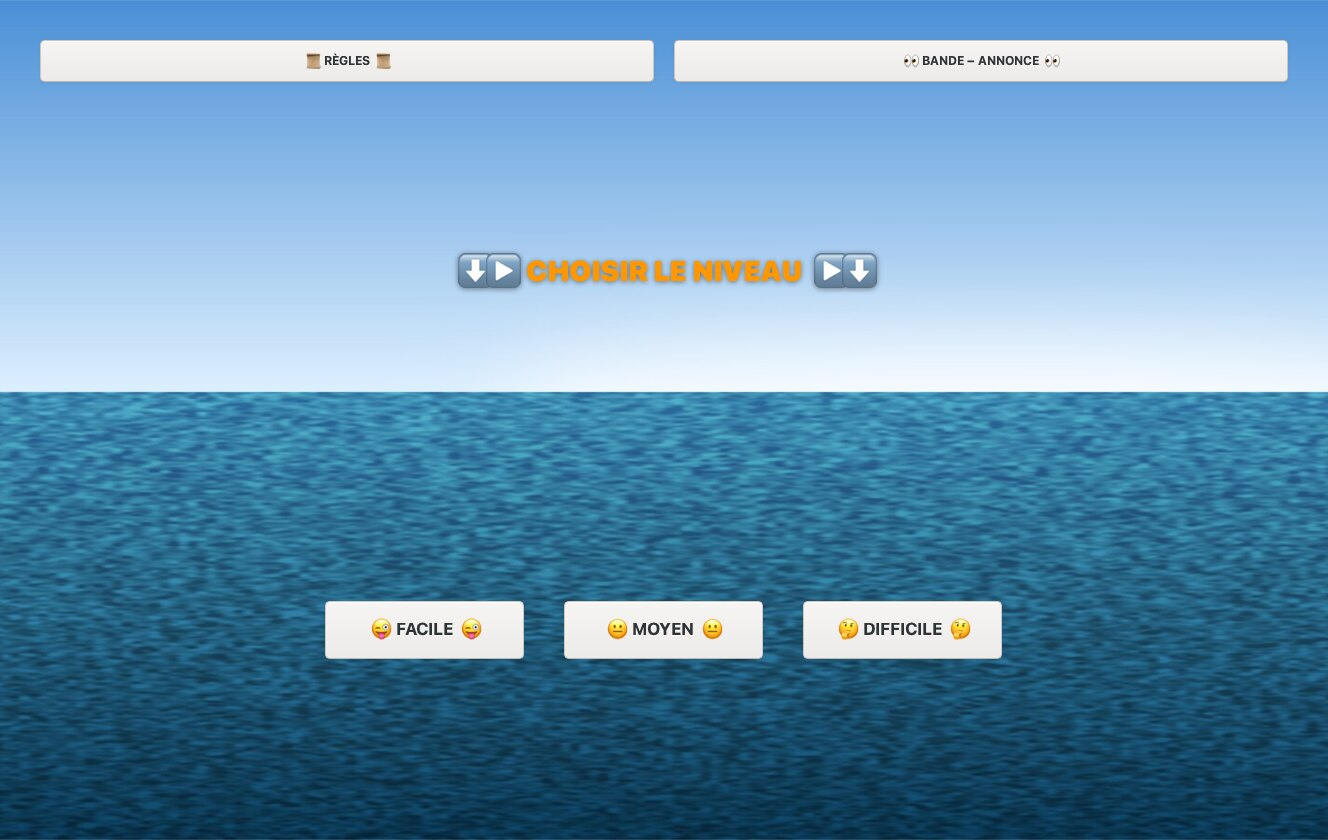
\includegraphics[width=0.78\textwidth]{../screenshots/menu.jpg}
    \caption{Version~2 --- choix du niveau.}
\end{figure}

\begin{figure}[H]
    \centering
    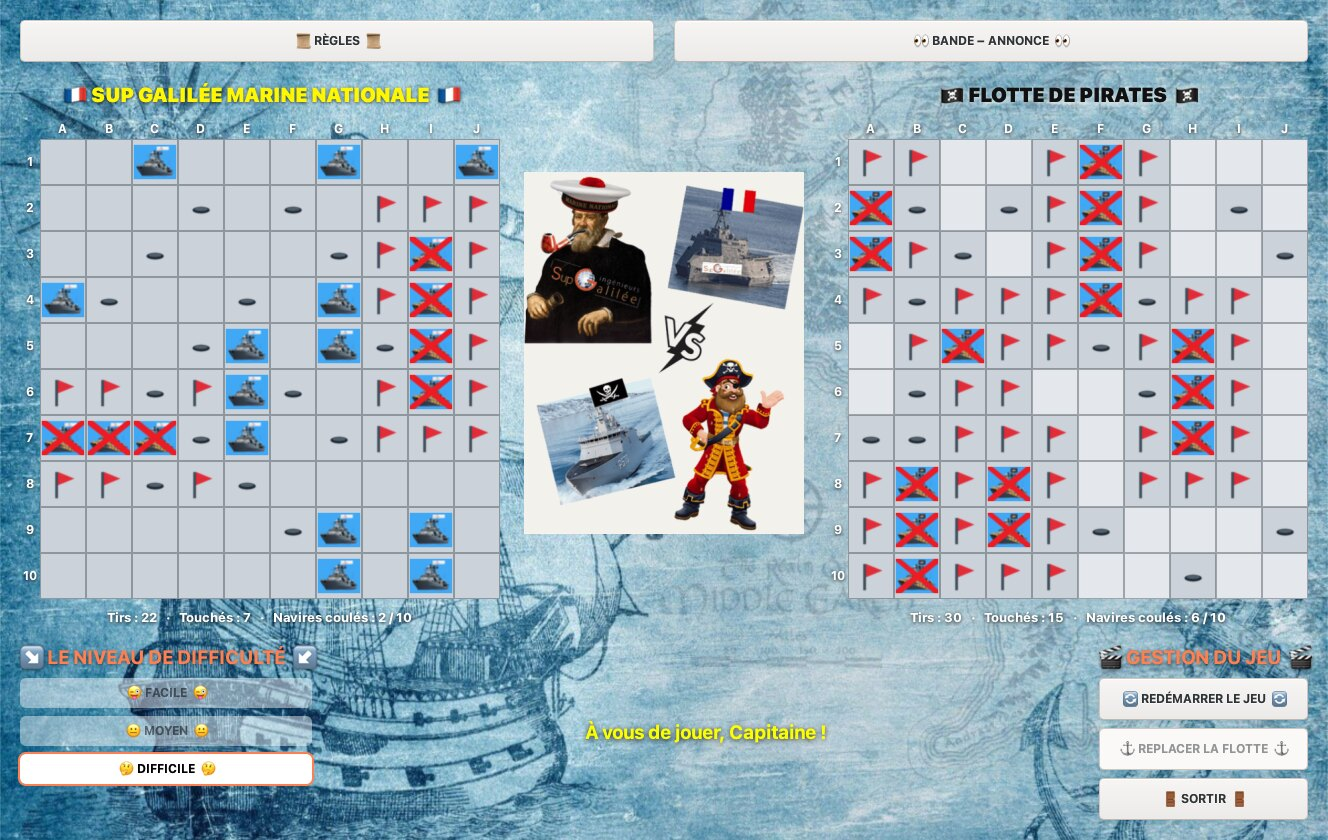
\includegraphics[width=\textwidth]{../screenshots/gameplay.jpg}
    \caption{Version~2 --- partie en cours au niveau difficile. À gauche, les drapeaux montrent
        ce que l'ordinateur a déduit ; à droite, ce que le joueur peut déduire.}
\end{figure}

\begin{figure}[H]
    \centering
    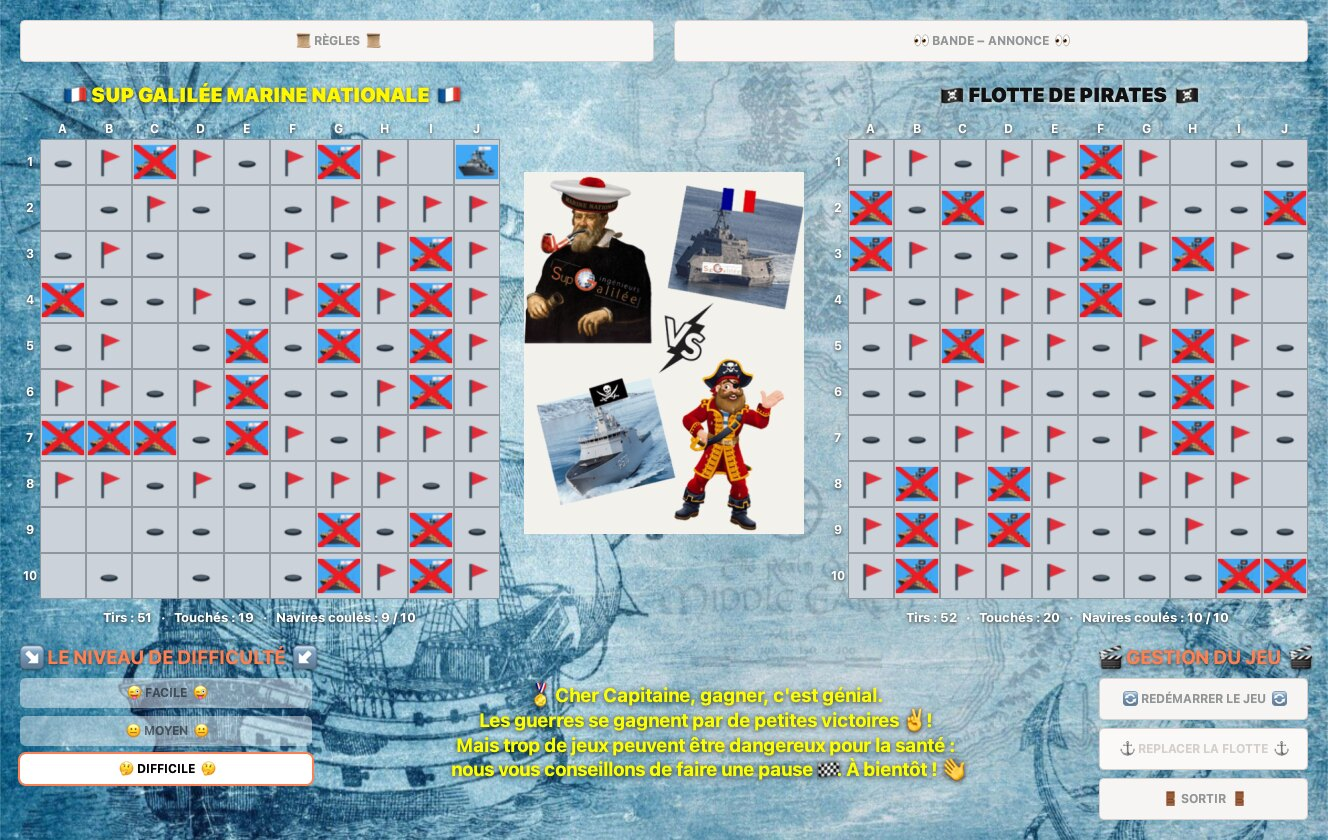
\includegraphics[width=\textwidth]{../screenshots/victory.jpg}
    \caption{Version~2 --- victoire.}
\end{figure}

\begin{figure}[H]
    \centering
    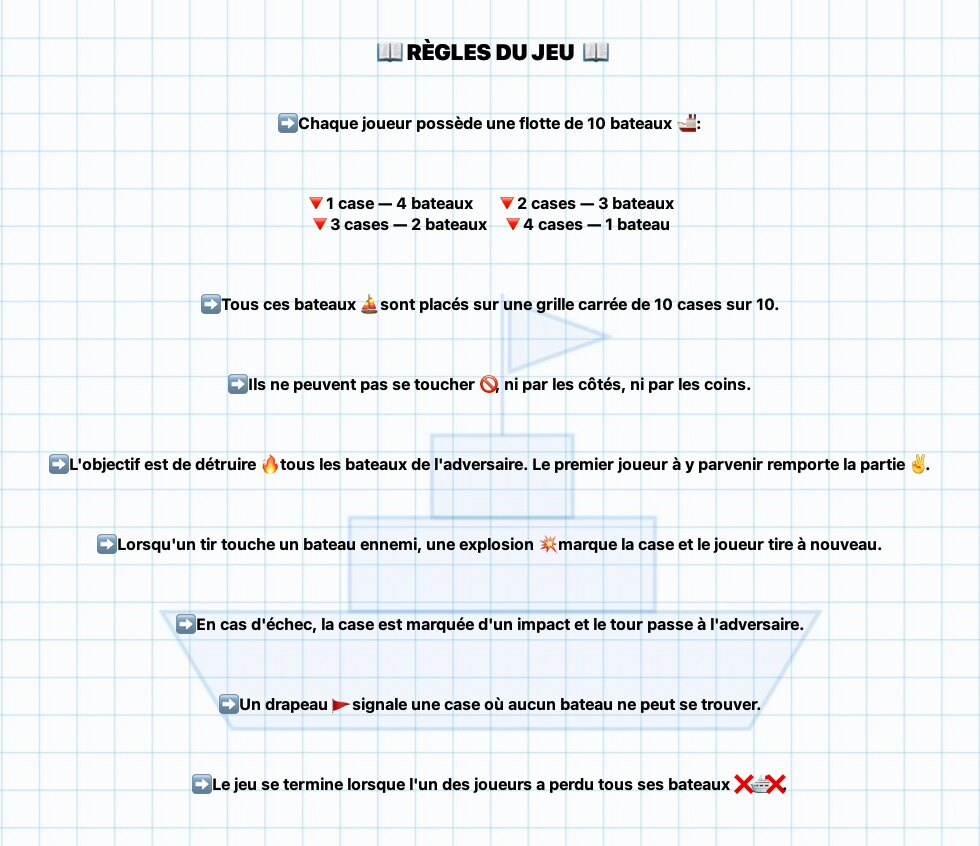
\includegraphics[width=0.8\textwidth]{../screenshots/rules.jpg}
    \caption{Version~2 --- fenêtre des règles.}
\end{figure}

\begin{figure}[H]
    \centering
    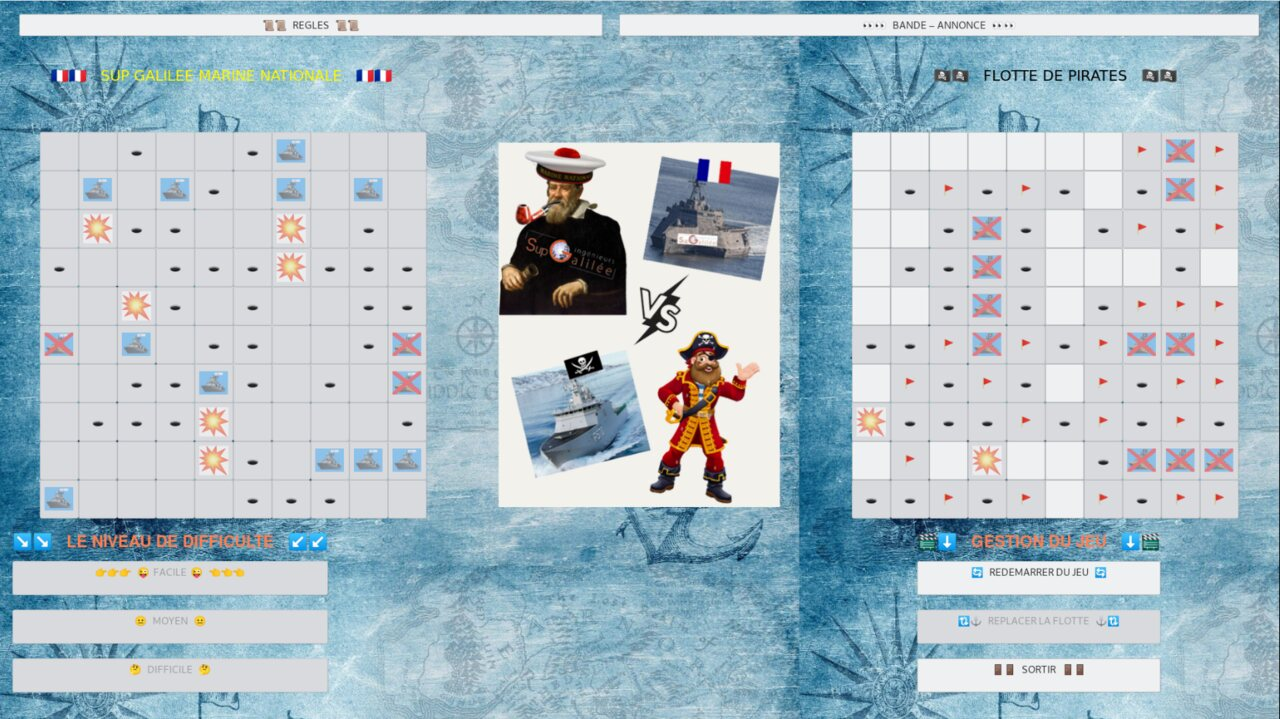
\includegraphics[width=\textwidth]{../screenshots/v1/gameplay.jpg}
    \caption{Version~1 (2023) --- partie en cours. L'identité visuelle a été conservée.}
\end{figure}


\printbibliography[title={Références}]

\end{document}
